\chapter{Veto efficiency studies for the 2024 WIMP search analysis}\label{chap:VetoEfficiency}
A WIMP scatter is expected to only deposit a small amount of energy (few~keV) within the LXe volume of the experiment in a single scatter. 
Neutrons produced through radioactive decays within detector materials mimics a WIMP interaction when they scatter off Xe atoms. Veto detectors surrounding the central LXe volume can detect these otherwise indistinguishable events and also permits assessment of the local radioactivity environment. A WIMP discovery will require excellent understanding of all background sources, which is best done through the characterization of those backgrounds \textit{in situ}. Efficiency of the veto systems in the detection of the radiation produced by the backgrounds should be maximised whilst minimizing the impact of the veto selection on detector livetime in turn maximising the detector livetime available for the detection of WIMPs. \autoref{sec:VetoEff/simulation_improvements} describes the series of improvements to the detector simulation geometry which were made prior to the WS2024 science run which aided the understanding of the response from the veto detector systems. The refinement of the veto selection algorithm is discussed alongside the impact that the veto selection had on the WS2024 result from \autoref{sec:VetoEff/VetoSelectionOptimisation} onwards.

\section{Improved Outer Detector Simulations}\label{sec:VetoEff/simulation_improvements}
The Outer Detector is defined as a Geant4 geometry, including transparency and other properties of each material, to allow simulations of neutron vetoes. 
Prior to WS2024 result, there were a number of major differences between simulations and data in the Outer Detector (OD). As such, an effort was made to correct this through modifications to the geometry of the Outer Detector in simulations to better reflect what is observed in data.
\subsection{Modifications of the Outer Detector simulation geometry}\label{sec:VetoEff/GeometryEdits}
There was a distinct discrepancy in neutron capture timing following single scatters within the TPC, this was one of the metrics which is investigated to quantify difference between data and simulation.
The simulation is improved through the following changes:
\begin{enumerate}
	%\item Spacing was added between the acrylic tanks to account for the gaps between the tanks which were present due to minor geometric differences produces in the moulding of the vessels during manufacturing process.
	\item Water was added to the foam volume which is between the OCV and acrylic tanks. The foam was intended to displace water to reduce neutron capture time, however the foam became saturated with water \footnote{A long-term bench top study found that samples of foam became saturated with water.}.
	\item The acrylic tanks were moved further away from the OCV in the simulation to reflect the actual position of the tanks in the Outer Detector, as installed.
\end{enumerate}
A series of simulations is produced varying both the amount of water saturation of foam displacer in 1\% steps and the position of the acrylic tanks from the OCV in 10~mm steps.
\begin{figure}[ht!]
	\centering
	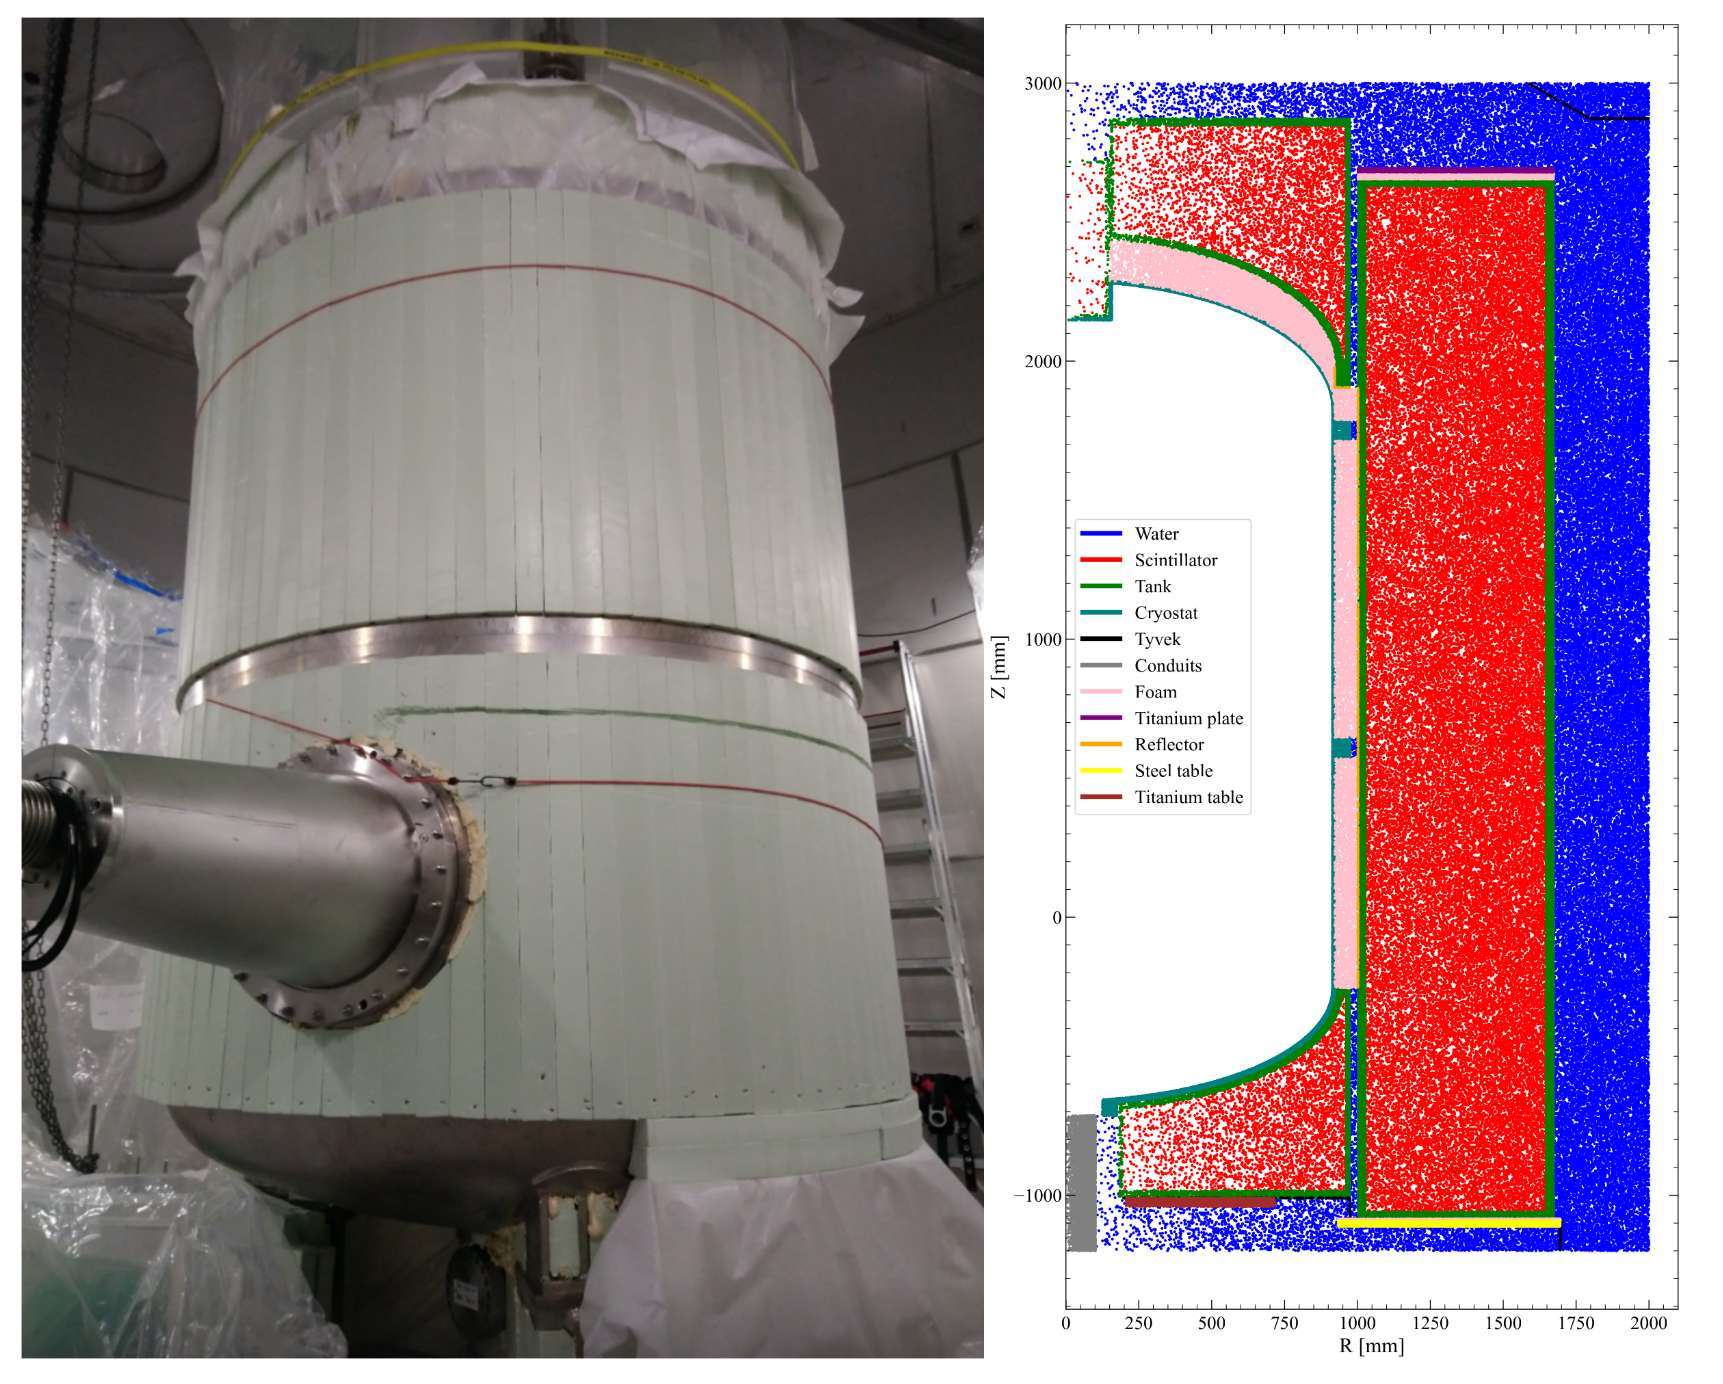
\includegraphics[width=0.9\textwidth]{figures/VetoEfficiency/FoamImgAndSimGeoTogether.png}
	\caption[An image of the foam displacer surrounding the OCS and final geometry in the simulation used for the WS2024 science run.]{Geometry in the simulation used for the WS2024 science run. \textbf{Left:} A photograph of the light green foam water displacer which resides between the acrylic tanks and the OCV. The water displacer was wrapped in a light reflector made from Tyvek. \textbf{Right:} A cross-section of the BACCARAT output. Geantinos (non-interacting test particles used for visualisation) were passed through the simulation geometry, the $xyz$ position information and Geant4 volumes were recorded to show the various volumes in the simulation.}
	\label{fig:VetoEff/od_geometry_for_sr3}
\end{figure}

Following these geometry changes, the neutron capture timing using AmLi is studied. Events which are classified as single scatters by LZap and pass the selection outlined in \autoref{sec:app/WSCoreCuts} are used for the study. OD pulses which exceeded a 200~keV (49~phd) threshold are used to optimise the geometry as corresponds to the threshold associated with proton recoil of neutrons of hydrogen in the OD medium.
All possible configurations of the geometry modifications are visually examined to determine which variation of simulation matches the data. An example of the comparison plot is shown in \autoref{fig:VetoEff/NC_AmLi_50mm7}, the "baseline simulation" is the initially configuration of the geometry prior to this study. %All plots were examined side by side in a large scale canvas configuration seen in Fig.\ref{fig:VetoEff/NC_Canvas0}, \ref{fig:VetoEff/NC_Canvas1}, \ref{fig:VetoEff/NC_Canvas2}, and \ref{fig:VetoEff/NC_Canvas3}. 
From this study it was found that 30~mm~to~50~mm movement of the SATs alongside 5\%~to~7\% increase in the percentage of water in the foam provides the best agreement between data and simulation at a 200~keV threshold. Including results from other studies on the H-Gd neutron capture ratios important when more water is present and thus more hydrogen, the \textit{best} configuration of the simulation geometry changes is found to be 30~mm and 6\% through matching the capture time of neutrons following single scatters in the active LXe volume.
\begin{figure}[!ht]
	\centering
	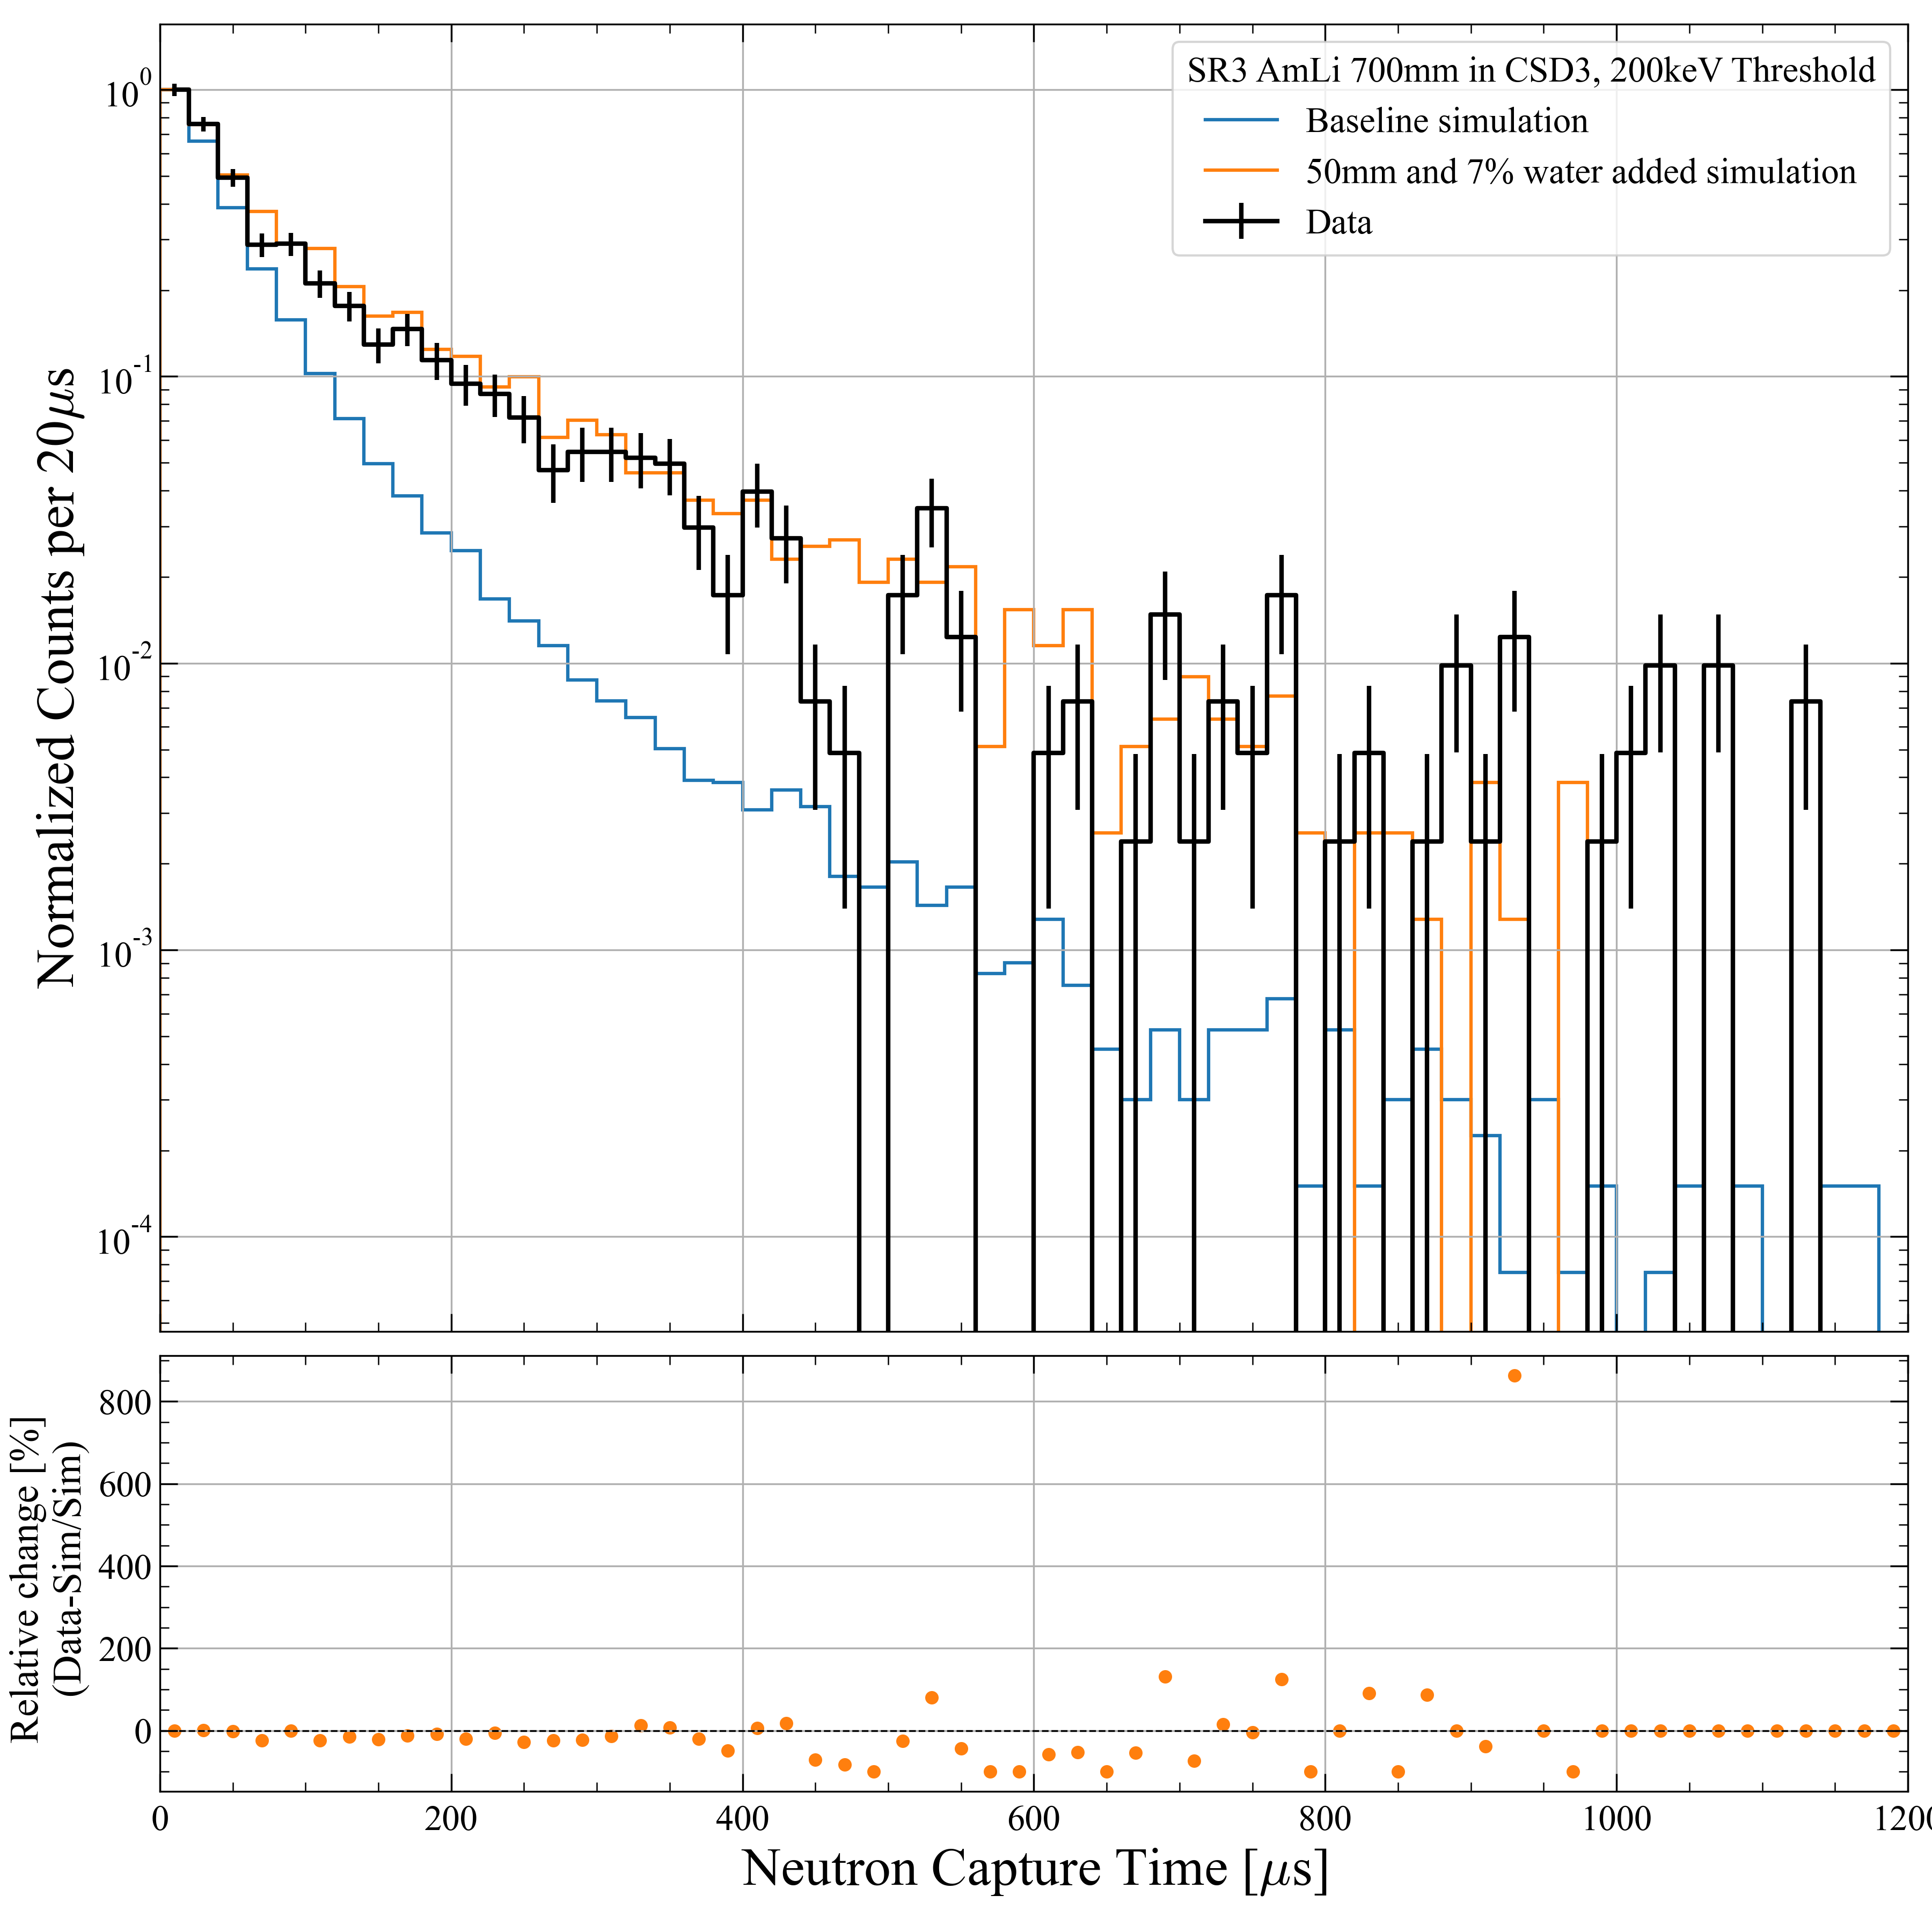
\includegraphics[width=0.7\linewidth]{figures/VetoEfficiency/movedSAT50mm_7percentWater_AmLi_CSD3_Z700mm_200keV_Ratio.png}
	\caption{An example of the plot used to compare neutron capture timing in data with the baseline simulation and the modified simulation. The relative change between data and simulation in each $20~\mu s$ bin is used to aid the visually examination across a 1200~\textmu s window.}
	\label{fig:VetoEff/NC_AmLi_50mm7}
\end{figure}

\section{Veto selection optimisation}\label{sec:VetoEff/VetoSelectionOptimisation}
A description of how the veto selection for the WS2024 is optimised is presented in this section. The Skin and OD veto cuts used in the WS2024 science run are based on those developed for the WS2022 science run, described in \cite{LZ:2022lsv} and are presented in \autoref{tab:VetoEff/sr3_veto_cuts}.
Both the OD and Skin detector may issue a veto and for each detector a tighter selection is defined for the first period after an interaction (\textit{prompt}) while a looser selection is applied for a longer time interval (\textit{delayed}) giving four veto categories each with their own intended purpose:
\begin{itemize}
	\item \textit{Skin-prompt} used for tagging $\gamma$-rays in the Skin detector
	\item \textit{OD-prompt} used for tagging $\gamma$-rays and neutron proton recoils in the OD
	\item \textit{Skin-delayed} used for tagging $\gamma$-rays from post-neutron capture de-excitation
	\item \textit{OD-delayed} used For tagging $\gamma$-rays from post-neutron capture de-excitation
\end{itemize}
The cuts used for the different veto criteria are selected at the same time as AmLi neutron tagging efficiency calculation, and are optimised to maximise the tagging efficiency whilst reducing deadtime. \textit{Pulse area} threshold, \textit{PMT coincidence} threshold and \textit{veto window length} are the three different variables which can be tuned for this optimisation. Events which were classified as single scatters by LZap and pass the selection outlined in \autoref{tab:VetoEff/amli_efficiency_cuts} are used for the study. The following subsections describe how each of the veto selection variables are tuned.

\begin{table}[!ht]
	\centering
	\caption{Outline of TPC cuts applied to AmLi calibration data for determining the veto efficiency. All cuts are defined in \autoref{sec:app/WSCoreCuts}.}
	\label{tab:VetoEff/amli_efficiency_cuts}
    \scalebox{0.9}{
	\begin{tabular}{llll}
    \hline\hline
    \textbf{Livetime cuts}&\textbf{Physics cuts}& \textbf{S2 cuts}& \textbf{S1 cuts}\\
    \hline
    Burst noise cut& Single scatter& S2 width vs drift time& S1 Stinger \\
    Muon holdoff& S1 threshold & Narrow S2& S1 TBA vs drift time\\
    Bad buffer cuts& S2 threshold& S2 rise time& S1 HSC \\
    Excess Area cut& Fiducial Volume& S2 early peak& S1 Shape\\
    & & S2 XY quality&\\
    & & S2 TBA &\\
    \hline\hline
	\end{tabular}}
\end{table}

\subsection{Veto window length}\label{sec:VetoEff/VetoWindowLength}
The veto window length is defined as the period of time after a single scatter in the TPC where a coincident signal in the OD or Skin would cause to reject the event.
The veto window length for the prompt windows are determined using AmLi and DD calibration data by measuring the time difference between the TPC single-scatter and OD and Skin pulses. The length of the prompt window is determined by width of the peak observed in the pulse timing distributions shown in \autoref{fig:VetoEff/veto_prompt_windows}. For the WS2024 selection, no change is made to the OD prompt veto window size, however the Skin prompt veto window is reduced by 500~ns as the pulses observed outside of the window $(0-250)$~ns are large enough to be rejected by the subsequent delayed veto and there are not pulses observed before $-250$~ns.
\begin{figure}[!ht]
	\centering
	\begin{subfigure}[b]{0.49\textwidth}
		\centering
		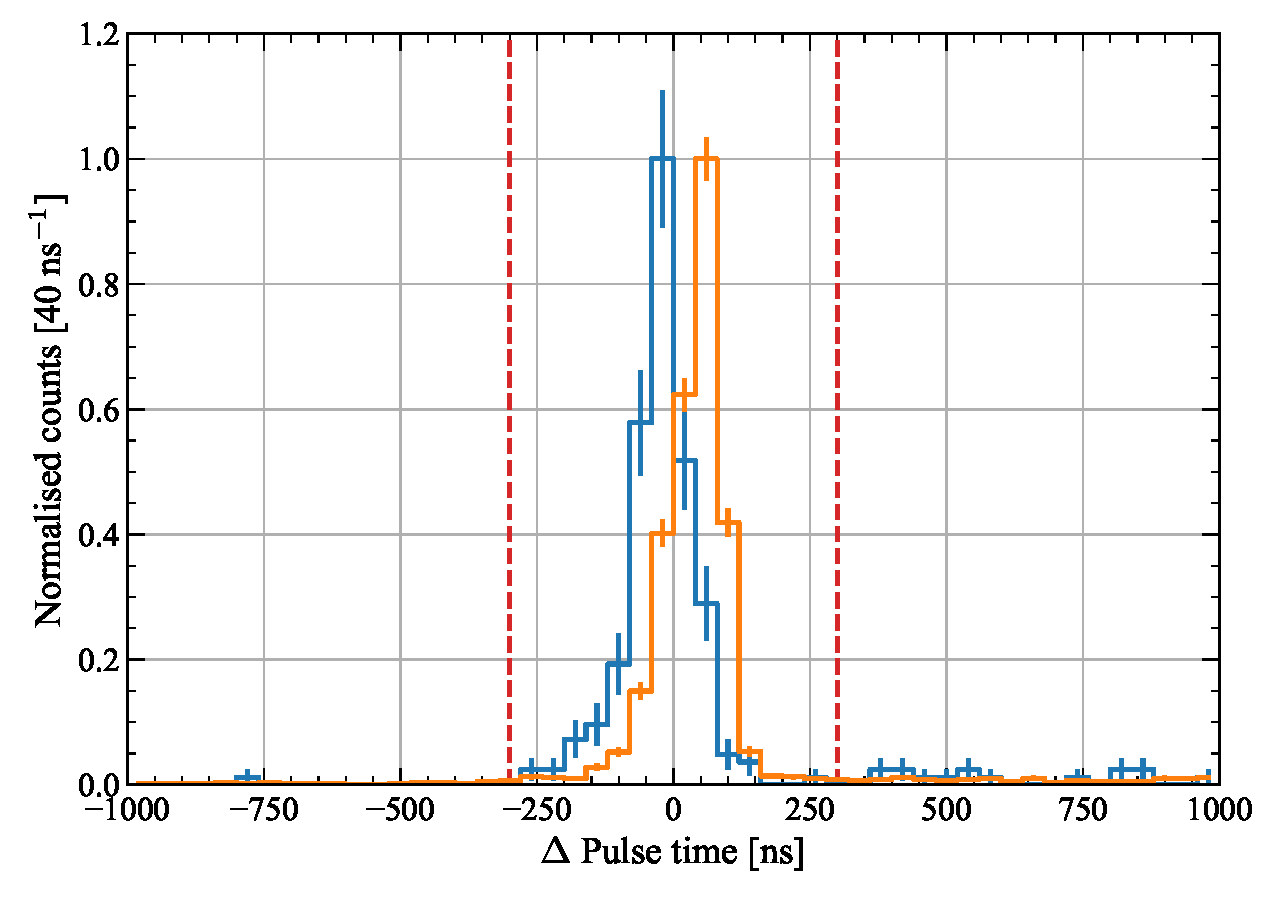
\includegraphics[width=\textwidth]{figures/VetoEfficiency/ODpromptWindowTiming.pdf}
		%\caption{Time difference (in ns) between TPC single-scatter and OD pulses using AmLi data.}
        \caption{}
		\label{fig:VetoEff/od_prompt_window}
	\end{subfigure}
	\hfill
	\begin{subfigure}[b]{0.49\textwidth}
		\centering
		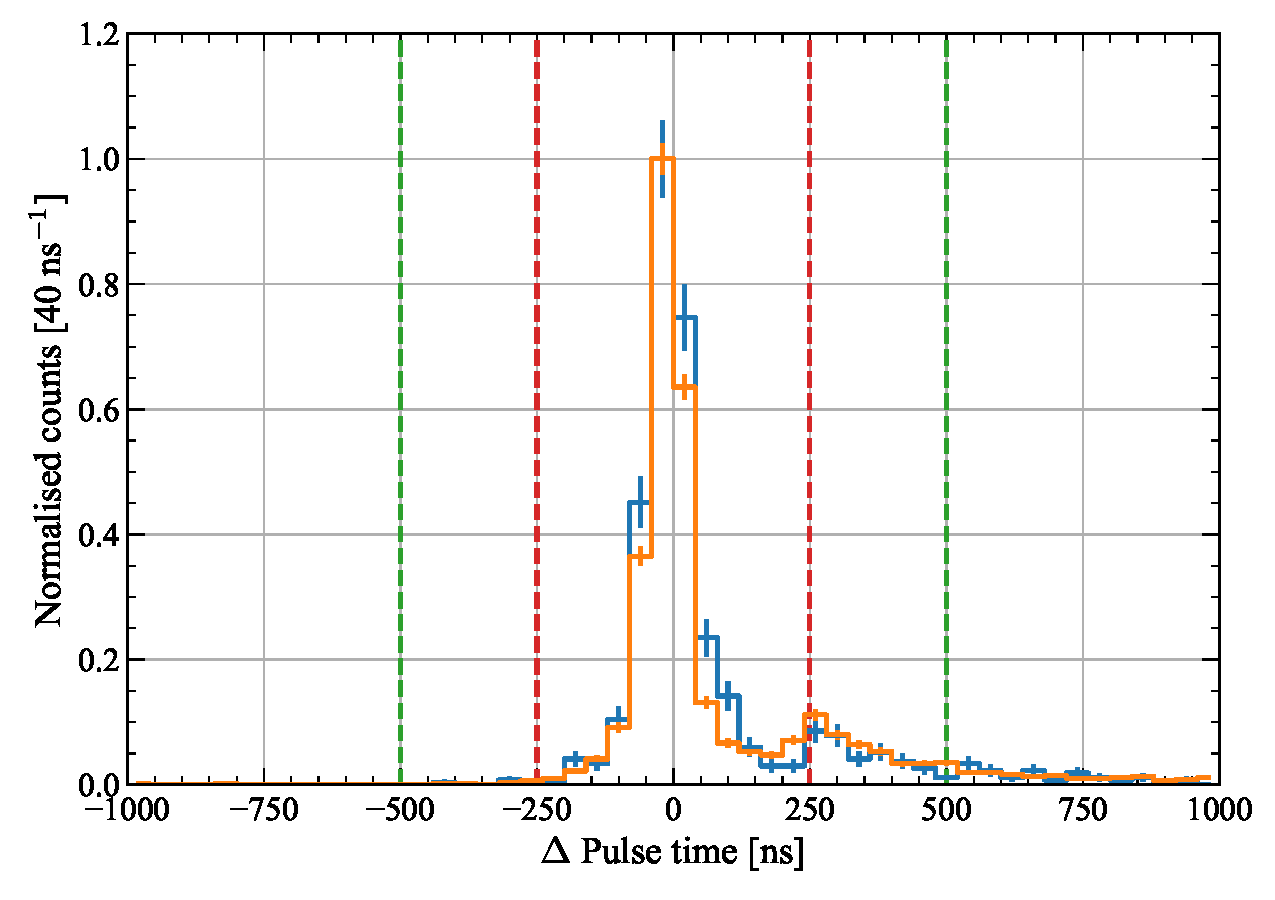
\includegraphics[width=\textwidth]{figures/VetoEfficiency/SkinpromptWindowTiming.pdf}
		%\caption{Time difference (in ns) between TPC single-scatter and OD pulses using DD data.}
		\caption{}
        \label{fig:VetoEff/skin_prompt_window}
	\end{subfigure}
	\caption{Prompt timing window for the OD (left) and Skin (right). %The time difference between TPC single scatter pulse and veto pulse was used to determine the optimal veto window size. 
    AmLi (blue) and DD (orange) calibration data was used to measure the time difference between the TPC single scatter pulse and veto pulse. 
    The vertical red lines indicate the boundary of the timing selection used for WS2024. There is no change in the size of the OD prompt veto window whereas the Skin prompt veto window is reduced by a total of 500~ns. The WS2022 veto window limits are shown in green.}
	\label{fig:VetoEff/veto_prompt_windows}
\end{figure}

The veto efficiency (defined in \ref{eqn:VetoEff/neutron_tagging_efficiency}) calculated using AmLi calibration data is used to determine the size of the delayed veto window for both the Skin and OD. The veto window length is reduced by a factor of two for both Skin and OD delayed windows as the slope of the efficiency curve begins to plateau above 600~\textmu s. An example of the veto efficiency plot used is shown in \autoref{fig:VetoEff/DelayedVetoWindow}.
\begin{figure}[!ht]
    \centering
    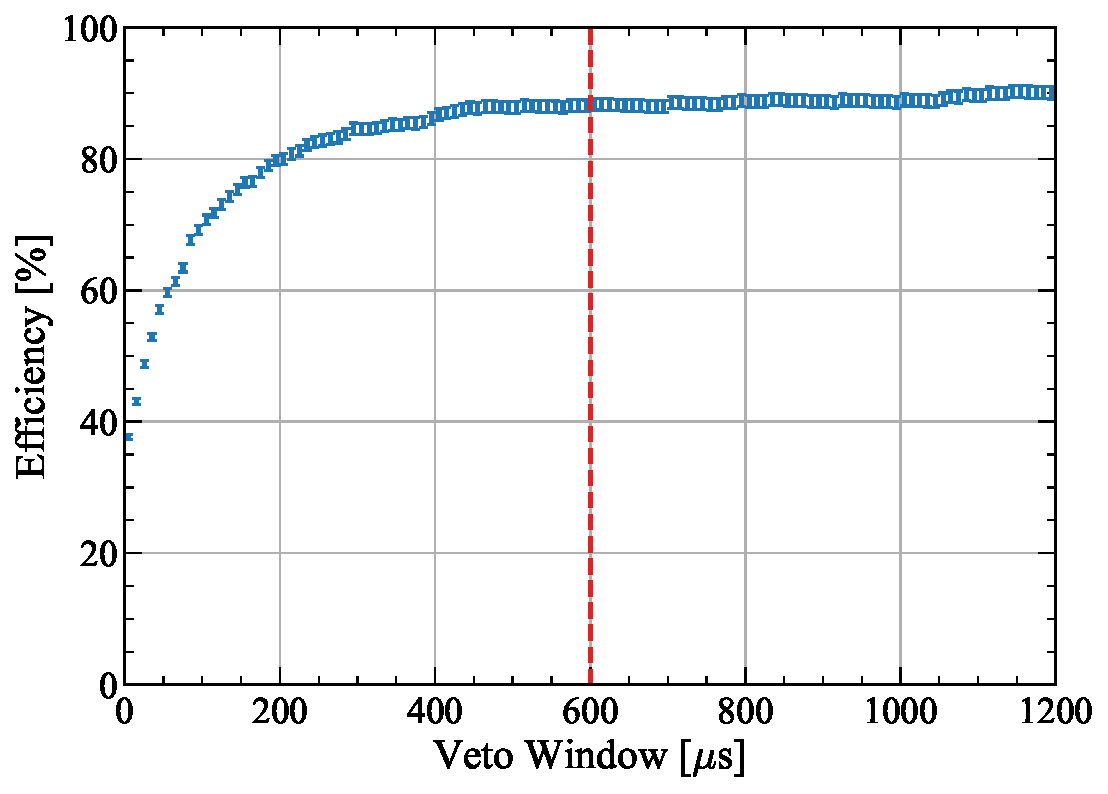
\includegraphics[width=0.7\linewidth]{figures/VetoEfficiency/DelayedVetoWindow.pdf}
    \caption{An example of a veto efficiency curve measured using AmLi calibration data. The vertical red line indicates the WS2024 upper bound of the delayed veto windows used for both the Skin and OD.}
    \label{fig:VetoEff/DelayedVetoWindow}
\end{figure}

The reduction in the veto window lengths has a positive impact on the dead time induced by the veto selection. Veto dead time is discussed in greater detail \autoref{sec:VetoEff/DeadtimeStability}.

\subsection{PMT Coincidence and pulse area threshold}
To optimize the pulse area and PMT coincidence thresholds the veto efficiency and deadtime is calculated for a grid in the pulse area and PMT coincidence requirement for the respective veto windows. An example of an efficiency grid (``heatmap'') is shown in \autoref{fig:VetoEff/od_prompt_veto_heatmap}. %All heatmaps produced for the optimization study are shown in \autoref{app:VetoHeatMapsSec}.

\begin{figure}
	\centering
	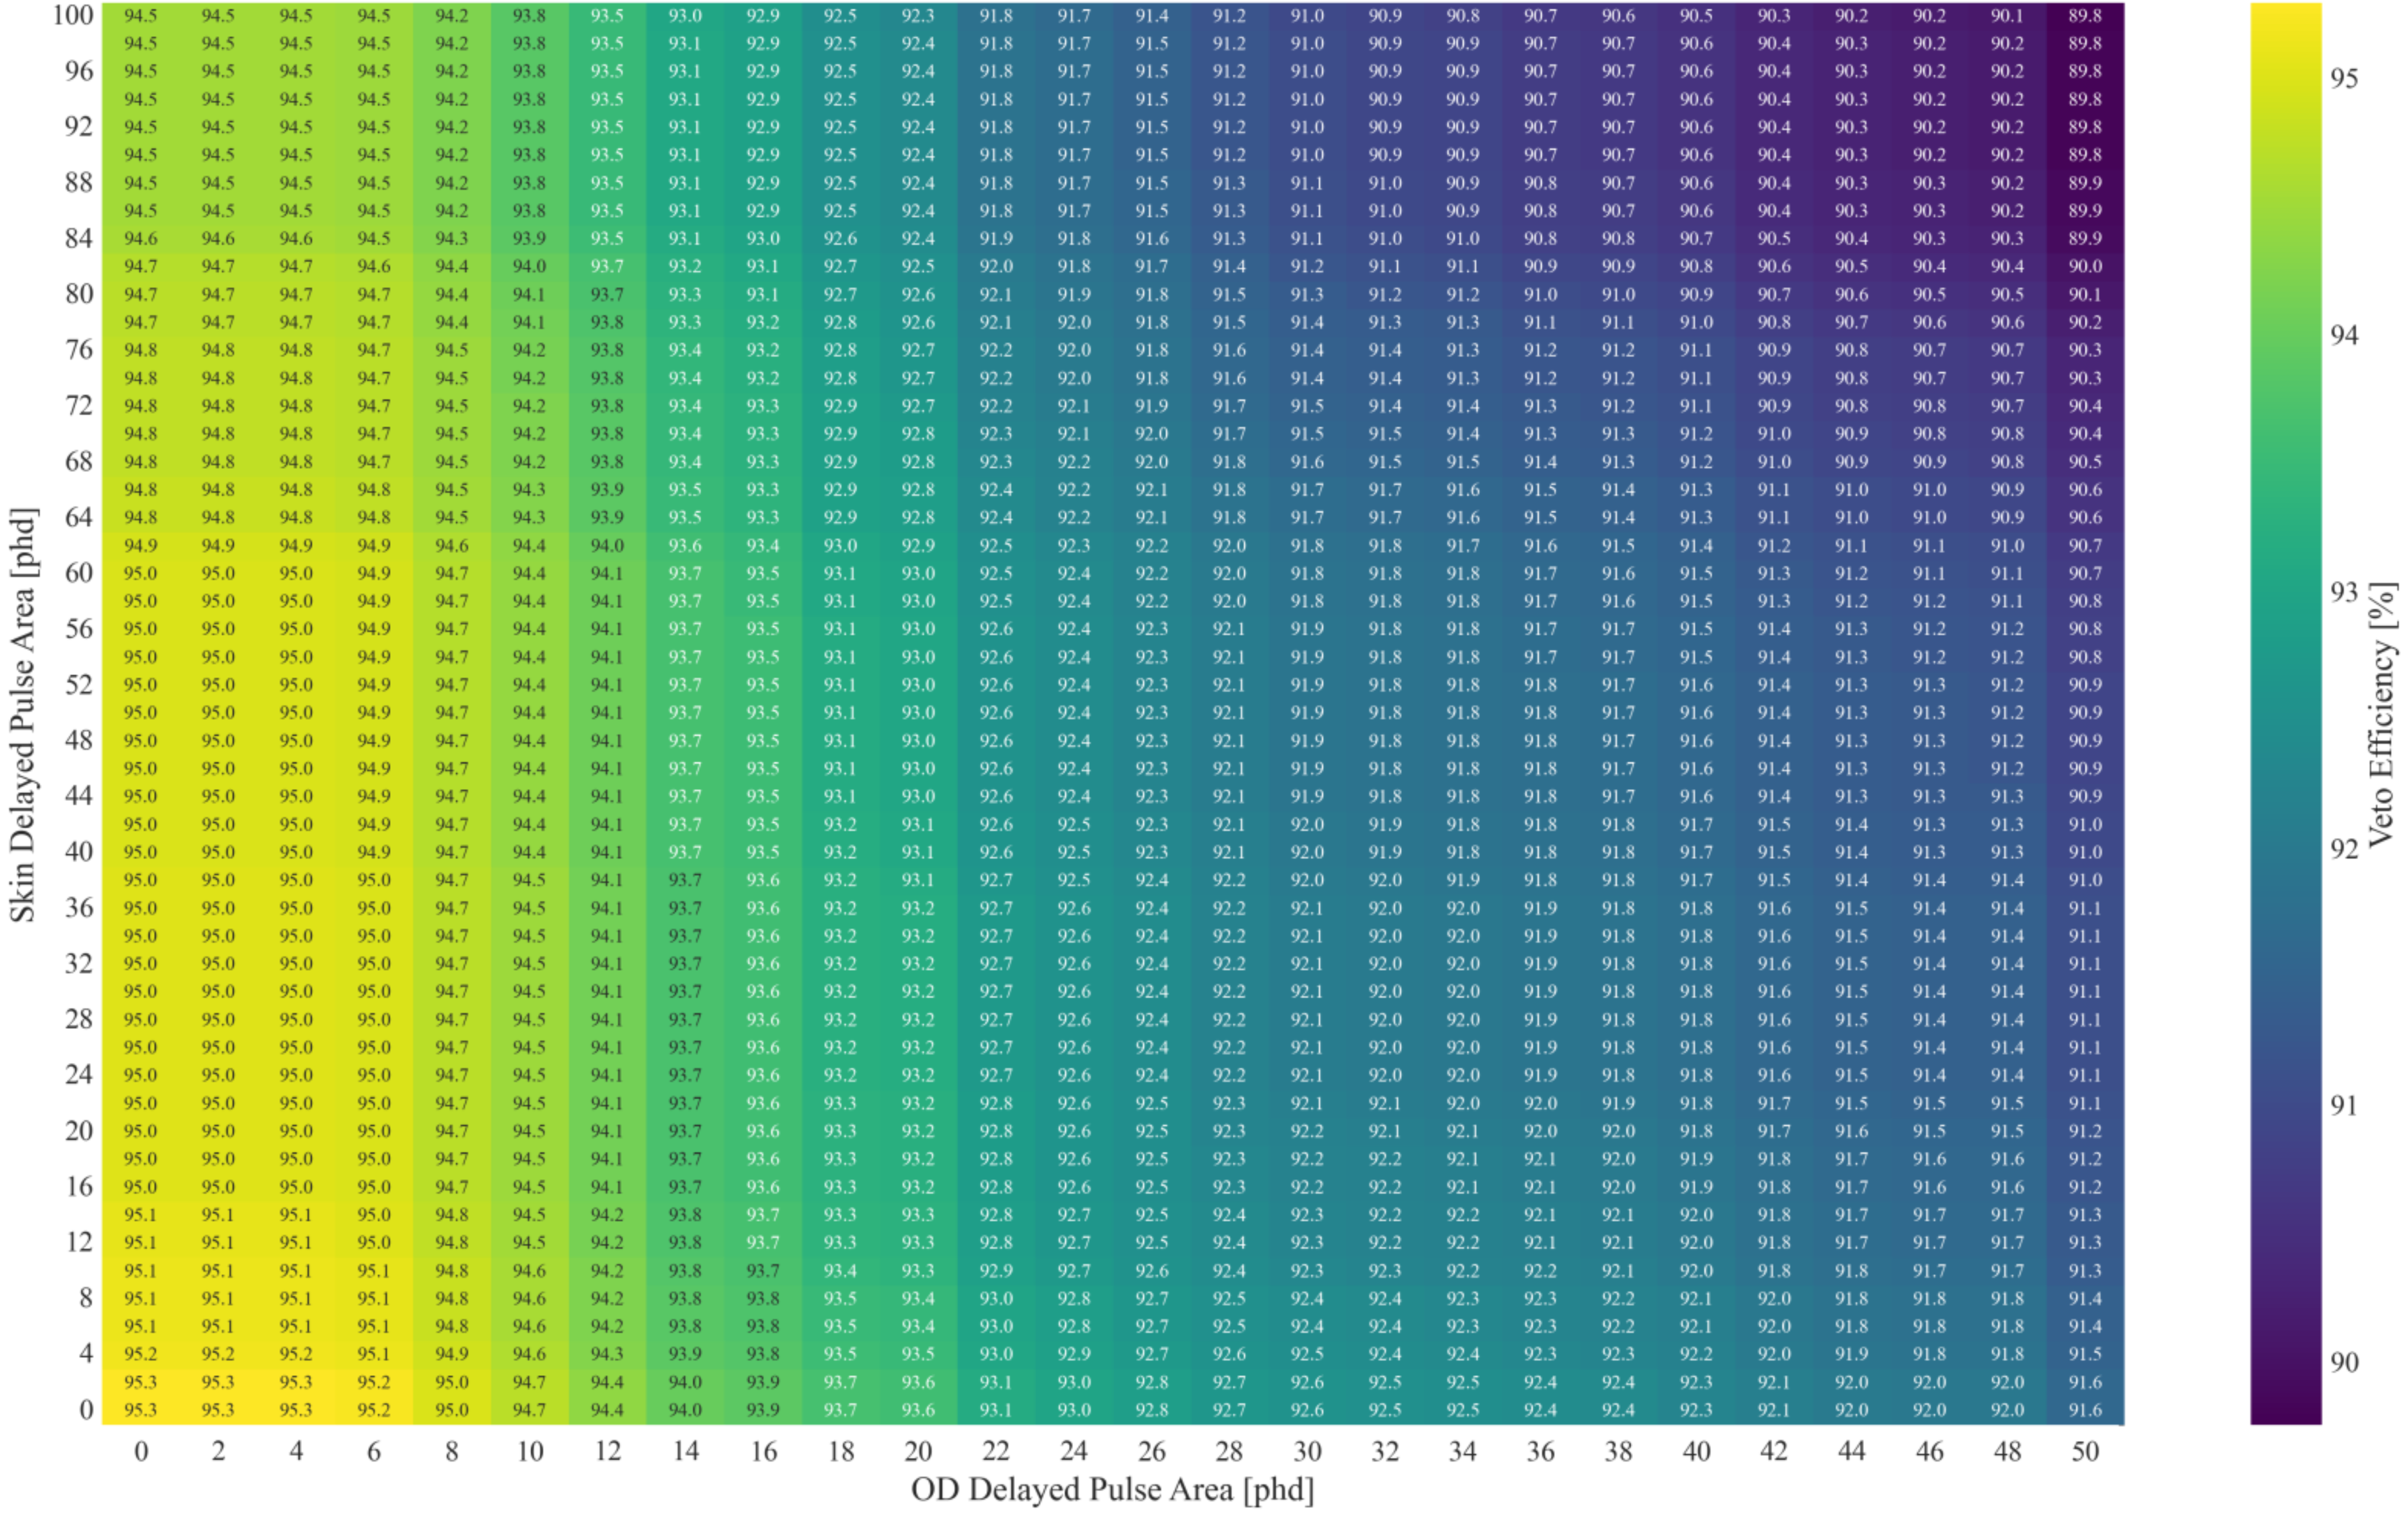
\includegraphics[width=\textwidth]{figures/VetoEfficiency/Heatmap600us_ODDelayedSkinDelayedThresholds.png}
	\caption{Heatmap used to determine optimal OD and Skin Delayed thresholds based on efficiency. The z-axis shows the efficiency associated with a given pulse area requirement for the delayed veto windows defined in \autoref{tab:VetoEff/sr3_veto_cuts}.}
	\label{fig:VetoEff/od_prompt_veto_heatmap}
\end{figure}

Compiling the heatmaps of efficiency and deadtime for established veto windows of the different criteria, thresholds are chosen to maximise efficiency whilst minimising dead time. An example plot used to determine this is shown in \autoref{fig:VetoEff/veto_cut_optimisation}.
For the WS2024 science run, the approach of trying to maintain the efficiency of WS2022 veto of $\sim$~89\%, whilst reducing the livetime impact is taken. It is determined that the efficiency can be matched to the veto efficiency achieved in the WS2022 science run whilst achieving a factor of two reduction in deadtime due to the tighter cuts obtained through better understand of the veto.

\noindent
The final cuts for the WS2024 science run are shown in \autoref{tab:VetoEff/sr3_veto_cuts}, with the WS2022 selection included for comparison. Any modifications to the selections are shaded to aid the readers eye.

\iffalse
\begin{sidewaysfigure}
	\centering
	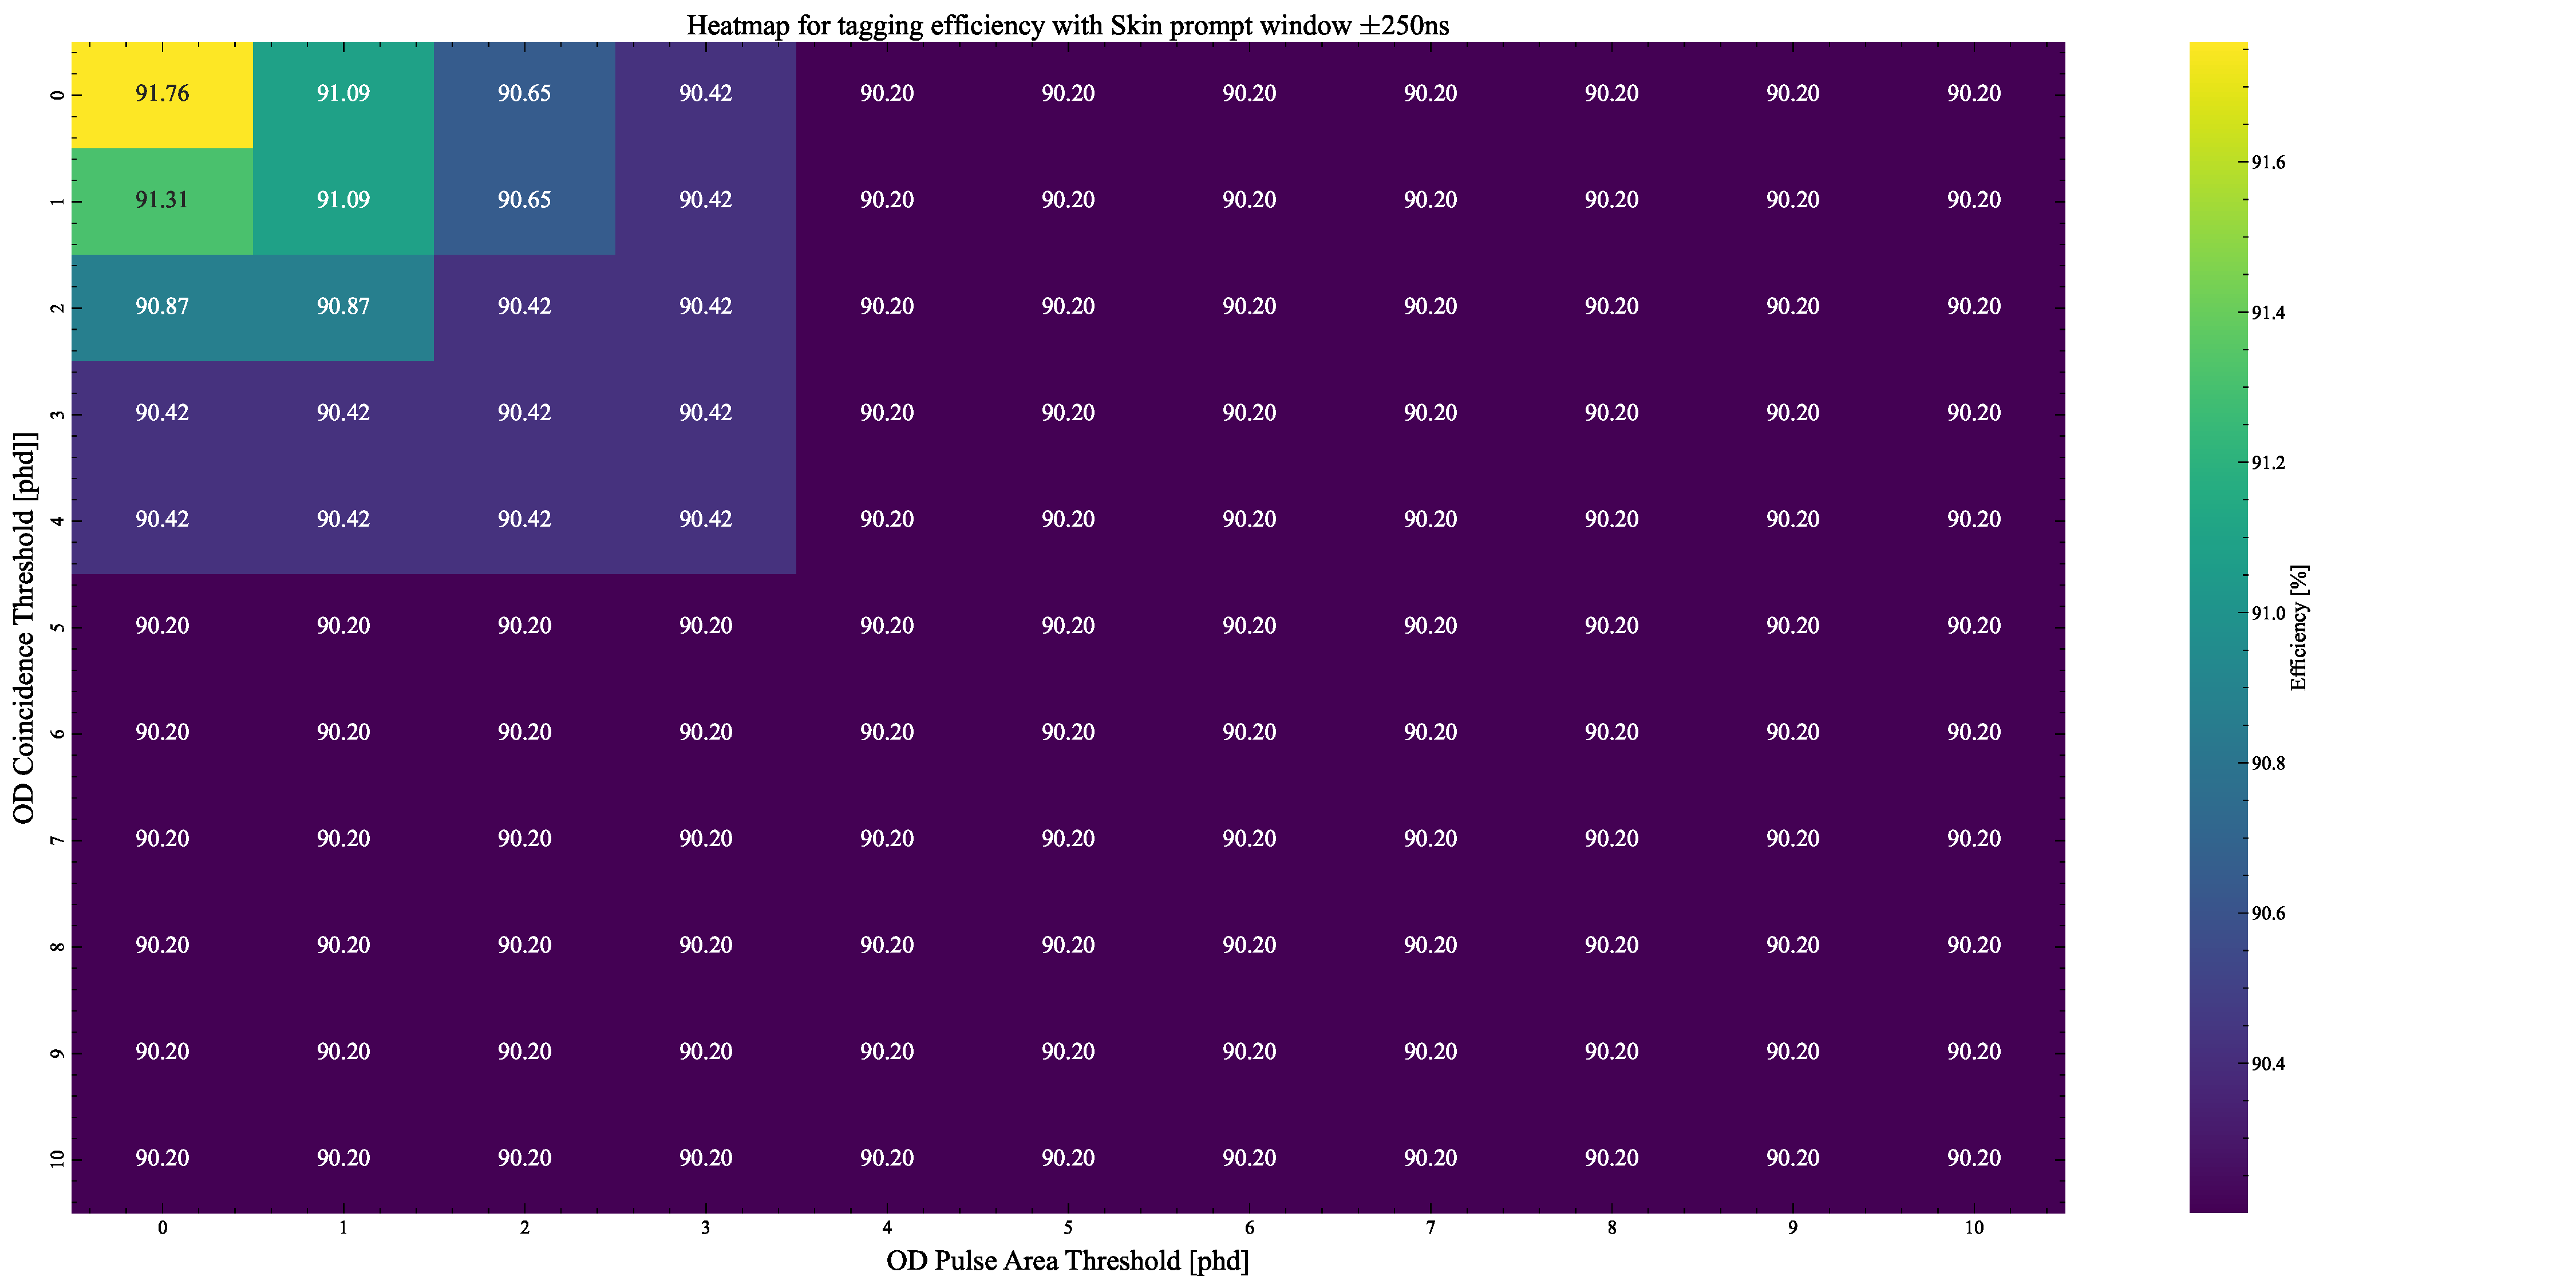
\includegraphics[width=\textwidth]{figures/VetoEfficiency/HeatmapSkinPACoinScanWindow500.pdf}
	\caption{Skin Prompt heatmap.
		In each bin, either the pulse coincidence or the pulse threshold has been varied.
		The z-axis shows the efficiency associated with a given pulse requirement.
		The veto time window considered is [-250, 250]ns.}
	\label{fig:VetoEff/skin_prompt_veto_heatmap}
\end{sidewaysfigure}
\begin{sidewaysfigure}
	\centering
	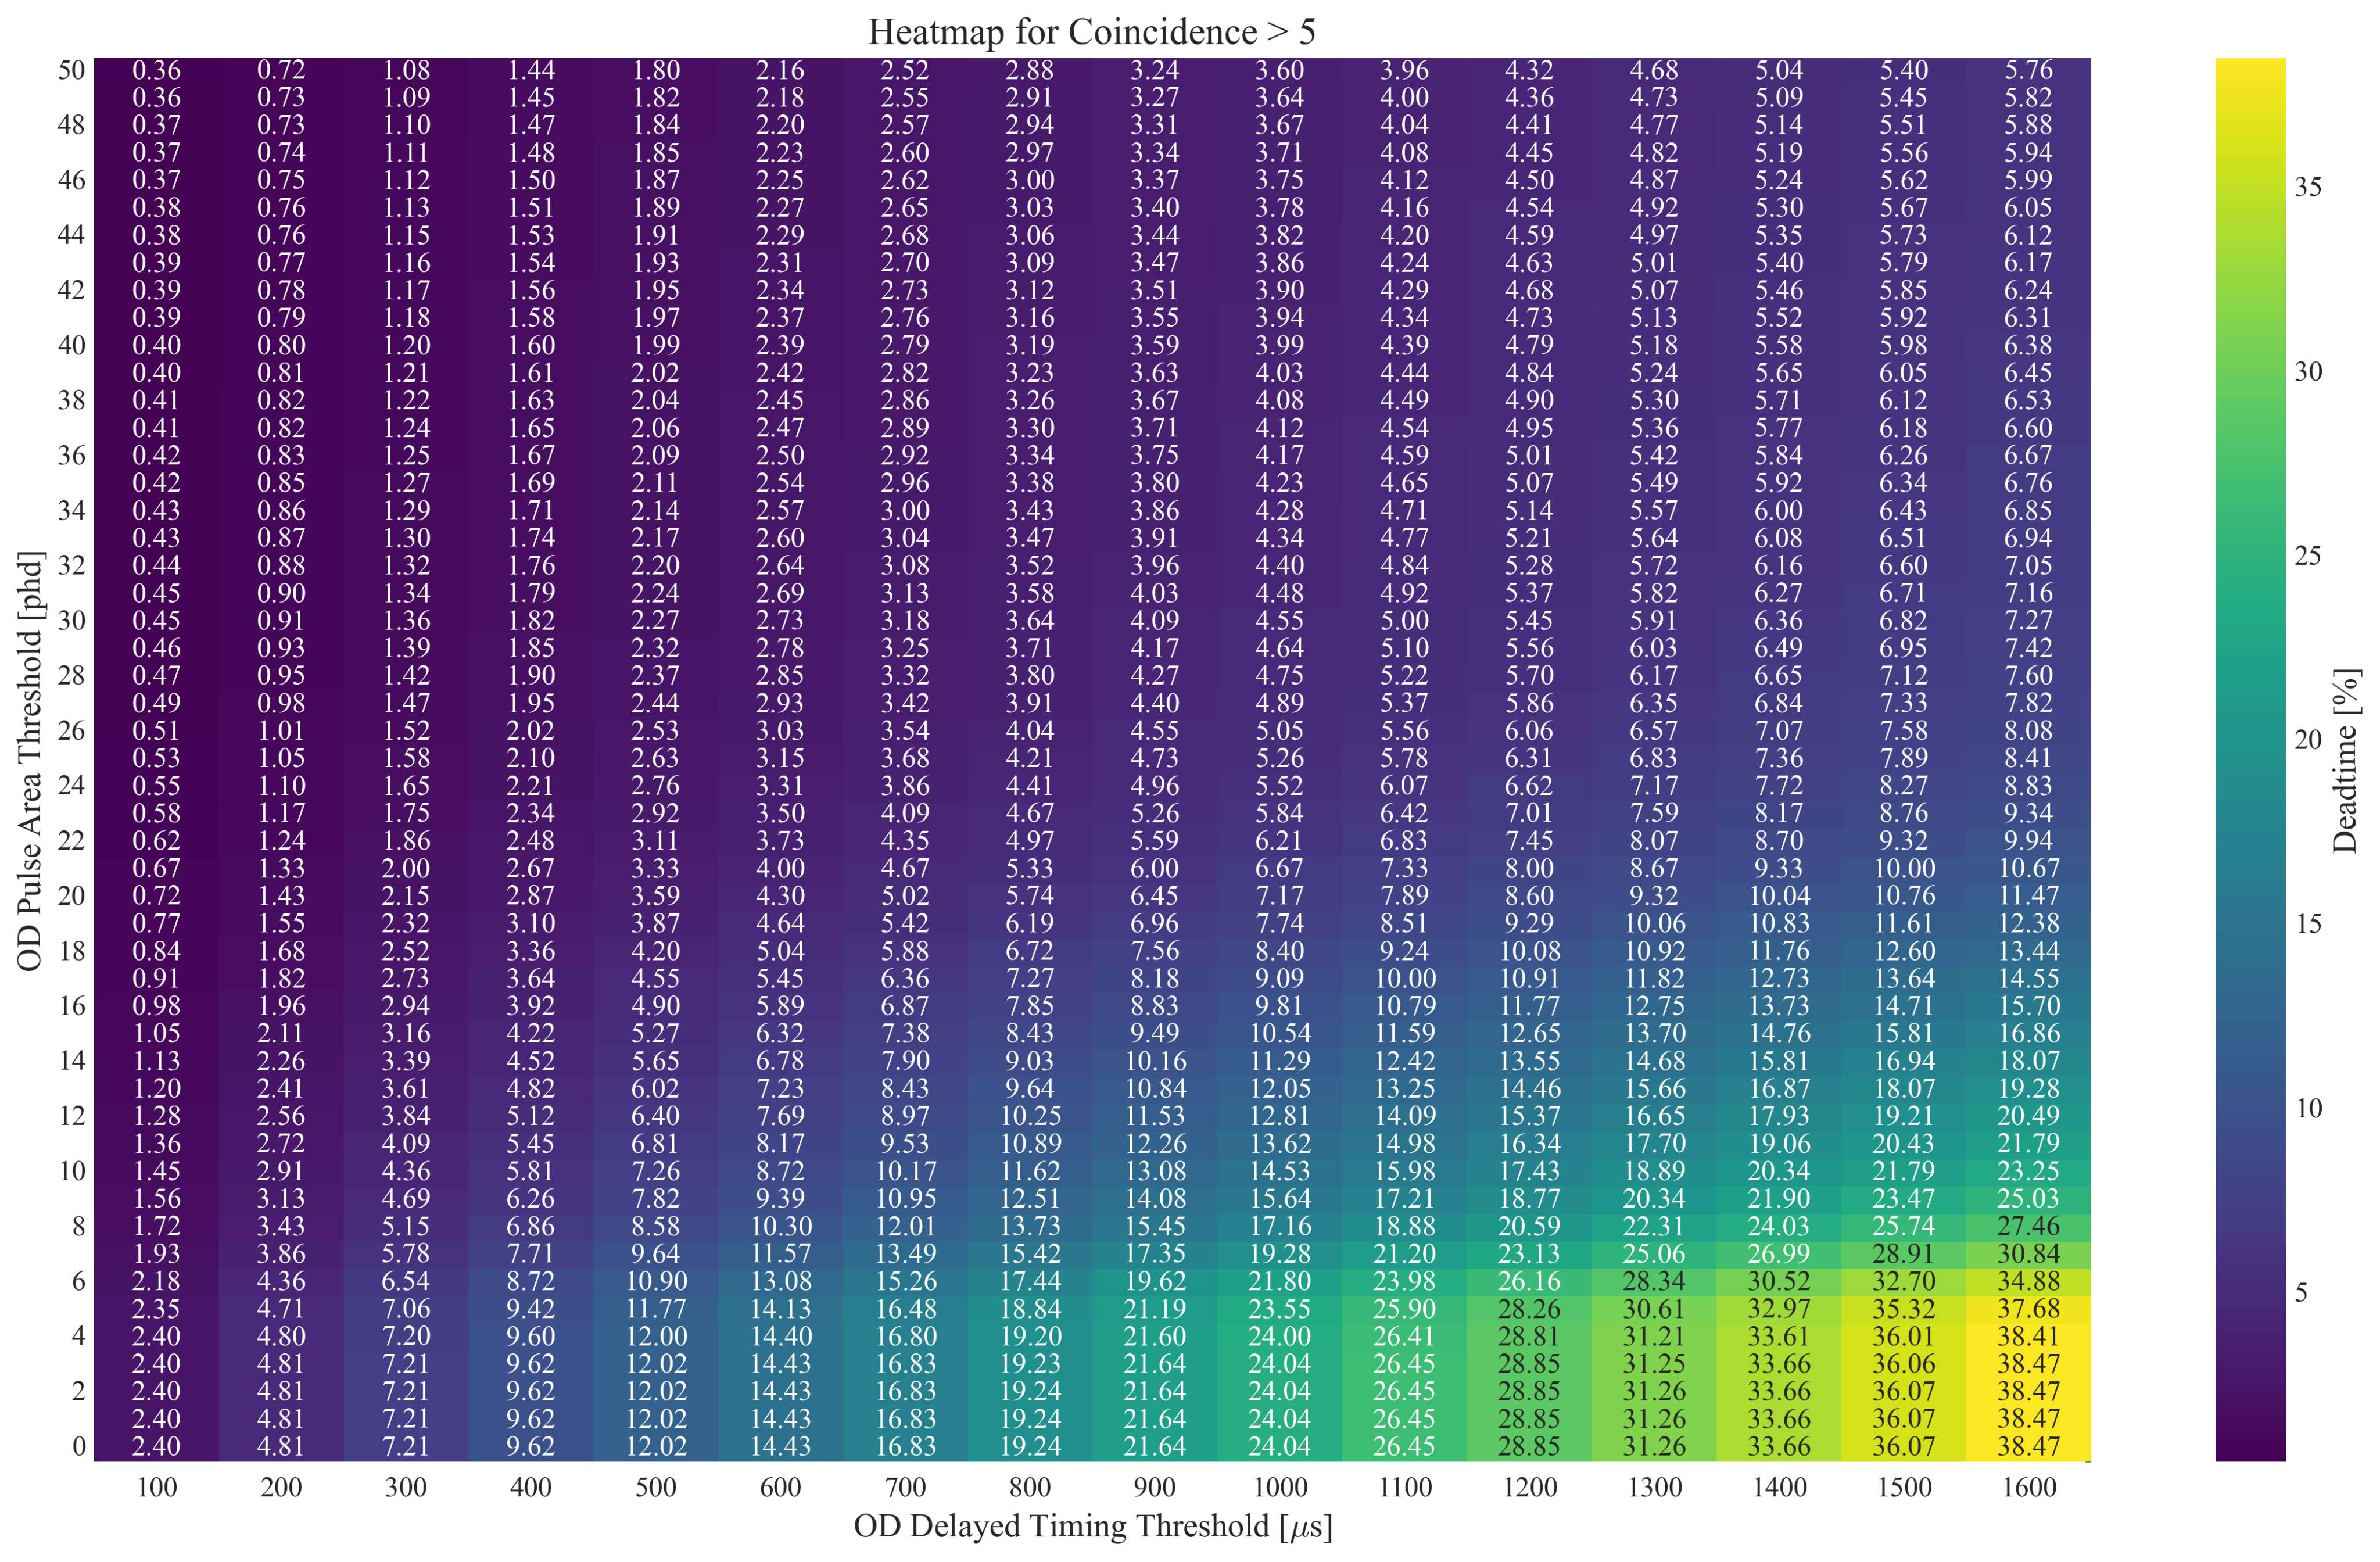
\includegraphics[width=\textwidth]{figures/VetoEfficiency/OD_Deadtime_thesis.png}
	\caption{OD Delayed heatmap.
		In each bin, either the veto window or the pulse threshold has been varied.
		The z-axis shows the deadtime associated with a given veto window and pulse threshold.
		In addition to the pulse area threshold, the pulse must have a coincidence greater than 5.}
	\label{fig:VetoEff/od_delayed_veto_heatmap}
\end{sidewaysfigure}
\begin{sidewaysfigure}
	\centering
	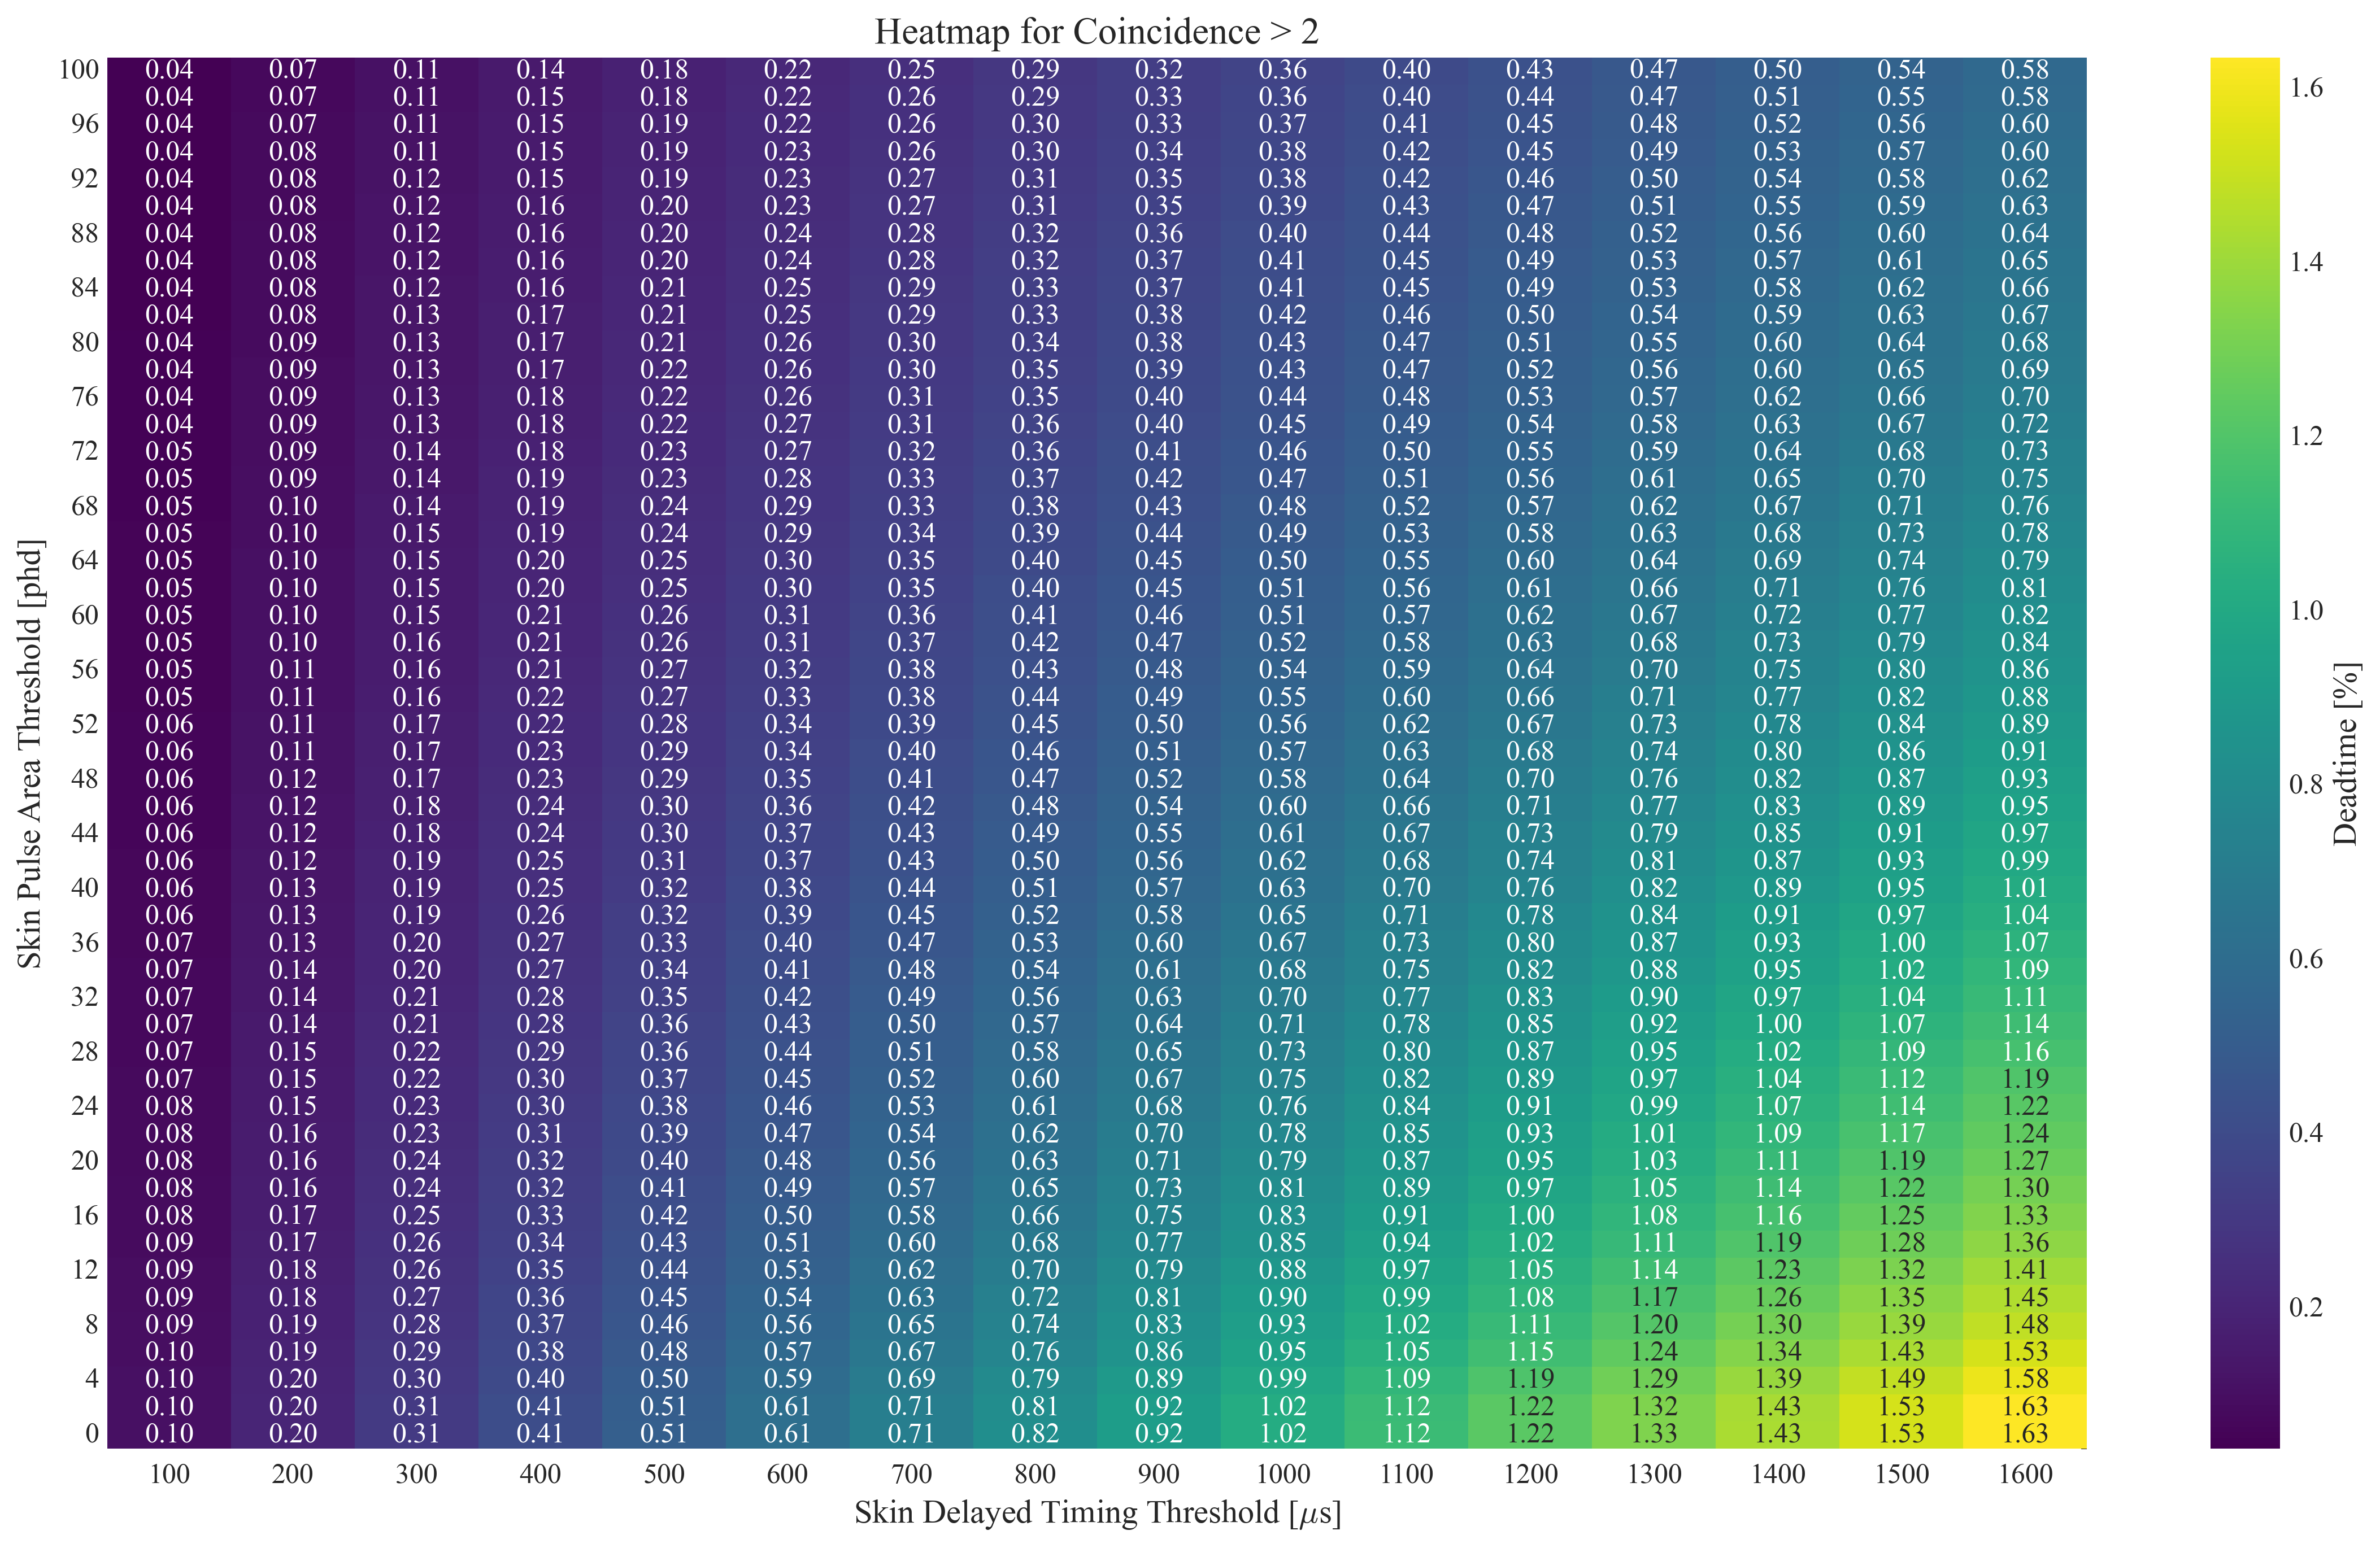
\includegraphics[width=\textwidth]{figures/VetoEfficiency/Skin_Deadtime_thesis.png}
	\caption{Delayed vetoes heatmap.
		In each bin, the OD pulse threshold or the Skin pulse threshold has been varied.
		The z-axis shows the veto efficiency associated with a given pulse thresholds.
		In addition to the pulse area threshold, the OD pulse must have a coincidence greater than 5, and the Skin pulse greater than 2.
		The veto window in this case is 500$\mu$s.}
	\label{fig:VetoEff/skin_delayed_veto_heatmap}
\end{sidewaysfigure}
\fi

\begin{figure}[!ht]
	\centering
	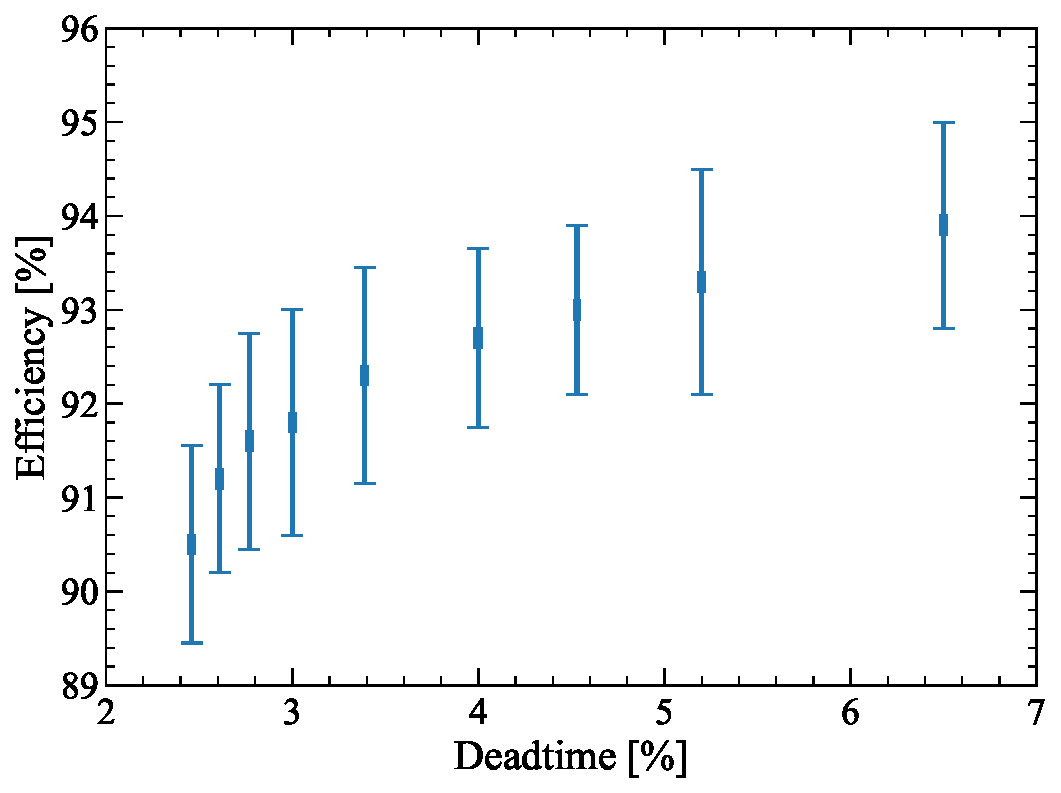
\includegraphics[width=0.7\textwidth]{figures/VetoEfficiency/DeadEffThresholdTest.pdf}
	\caption[Example plot used to highlight a number of considered cuts for the delayed Skin and OD pulse area thresholds for a 600~$\mu$s window.]{Example plot used to highlight a number of considered cuts for the delayed Skin and OD pulse area thresholds for a 600~$\mu$s window. The efficiency values have not been corrected for accidental coincidences. At each point, the numbers in brackets are the OD threshold pulse area, and the Skin threshold pulse area.}
	\label{fig:VetoEff/veto_cut_optimisation}
\end{figure}

\iffalse
\begin{figure}[!ht]
	\centering
	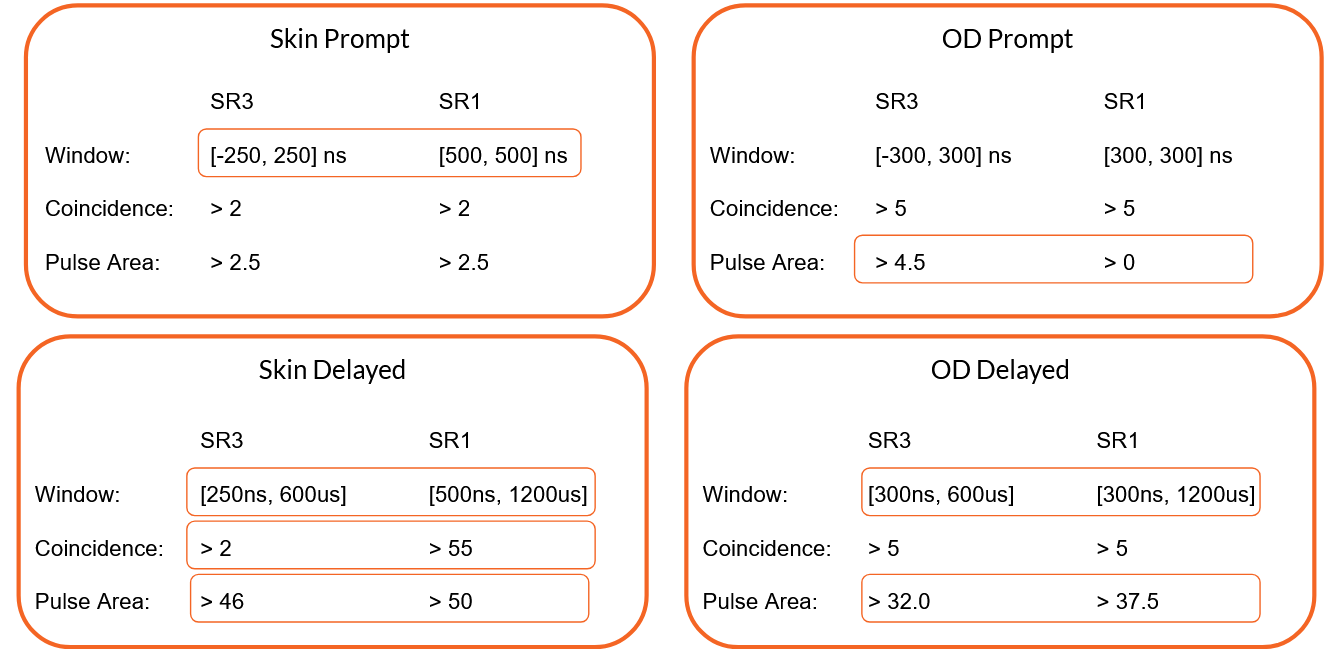
\includegraphics[width=0.9\textwidth]{figures/VetoEfficiency/sr3_cuts.png}
	\caption{Cuts determined to be optimal for the WS2024 science run.
		The WS2022 cuts are also included, where any modifications made to the selections is highlight accordingly.}
	\label{fig:VetoEff/sr3_veto_cuts}
\end{figure}
\fi

\begin{table}[!ht]
    \centering
    \caption{Cuts determined to be optimal for the WS2024 science run. The WS2022 cuts are also included, where any modifications made to the selections is shaded accordingly.}
    \label{tab:VetoEff/sr3_veto_cuts}
    \scalebox{0.9}{
    \begin{tabular}{|c|c|c||c|c|c|}
    \hline
    \multicolumn{3}{|c||}{\textbf{Skin Prompt}} & \multicolumn{3}{c|}{\textbf{OD Prompt}} \\
    \hline
    & WS2024 & WS2022 & & WS2024 & WS2022 \\
    \hline
    Window & \cellcolor[HTML]{cecece} [-250,250]~ns & \cellcolor[HTML]{cecece}[500,500]~ns & Window & [-300,300]~ns & [-300,300]~ns\\
    Coincidence&$>2$&$>2$&Coincidence&$>5$&$>5$\\
    Pulse Area & $>2.5$ & $>2.5$ & Pulse Area & \cellcolor[HTML]{cecece}$>4.5$ &\cellcolor[HTML]{cecece} $>0$ \\    
    \hhline{|===||===|}
    \multicolumn{3}{|c||}{\textbf{Skin Delayed}} & \multicolumn{3}{c|}{\textbf{OD Delayed}} \\
    \hline
    &WS2024&WS2022&&WS2024&WS2022\\
    \hline
    Window&\cellcolor[HTML]{cecece}[250~ns, 600~$\mu$s]&\cellcolor[HTML]{cecece}[500~ns, 1200~$\mu$s]&Window&\cellcolor[HTML]{cecece}[300~ns, 600~$\mu$s]&\cellcolor[HTML]{cecece}[300~ns, 1200~$\mu$s]\\
    Coincidence&\cellcolor[HTML]{cecece}$>2$&\cellcolor[HTML]{cecece}$>55$&Coincidence&$>5$&$>5$\\
    Pulse Area&\cellcolor[HTML]{cecece}$>46$&\cellcolor[HTML]{cecece}$>50$&Pulse Area&\cellcolor[HTML]{cecece}$>32.0$&\cellcolor[HTML]{cecece}$>37.5$\\
    \hline
    \end{tabular}}
\end{table}

\subsection{Deadtime stability}\label{sec:VetoEff/DeadtimeStability}
The stability of the induced deadtime for each of the veto selection windows over the WS2024 science run is assessed for stability by comparing the deadtime at monthly intervals. For each month, the rate of pulses in the Skin and OD, using randomly triggered data; and the rate above the threshold, defined by the specific veto cut, is recorded. The stability of measured deadtime over the WS2024 science run is shown in \autoref{fig:VetoEff/deadtime_stability}.
The deadtime is then calculated as:
\begin{equation}
	\textrm{Dead Time [\%]} = 100 - (\lambda(x)\cdot t_{\text{vw}})
\end{equation}
where $\lambda(x)$ is the background rate above the veto threshold $x$, and $t_{\text{vw}}$ represents the veto window length measured in ns.
The conclusion that the deadtime is stable over the WS2024 science run is confirmed by measuring the rate of OD pulses above $200~\text{keV}$ (as defined by the WS2022 energy calibration) using the \lstinline{ODHealth} PREM module. No significant fluctuation is observed during WS2024 science run, shown in \autoref{fig:VetoEff/deadtime_stability_prem}.
\begin{figure}[!ht]
	\centering
	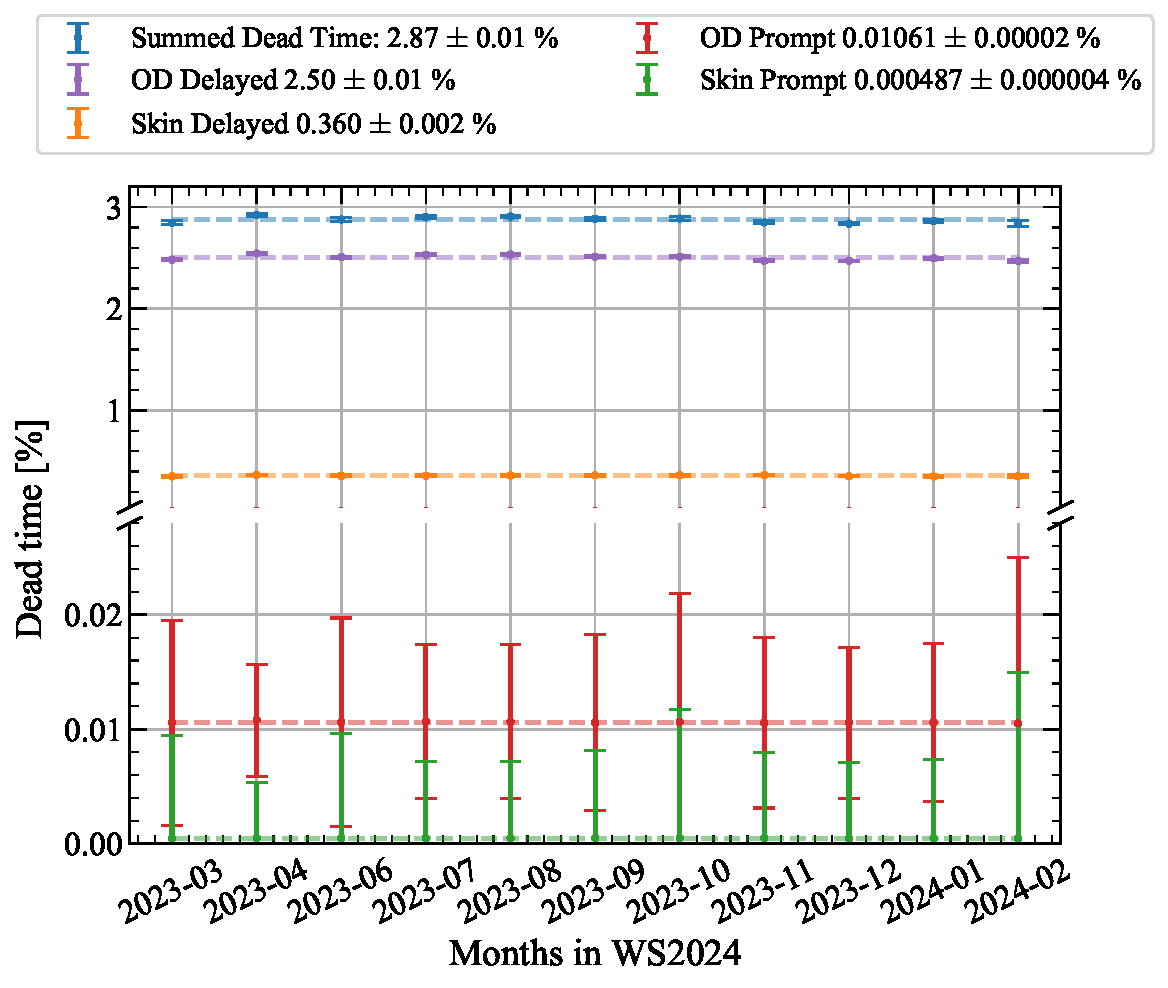
\includegraphics[width=0.7\textwidth]{figures/VetoEfficiency/SR3DeadTimeAll_withMean.pdf}
	\caption[Deadtime from the Skin and OD veto selection criteria during each month of WS2024 science run.]{Deadtime from the Skin and OD veto selection criteria during each month of WS2024 science run. The error shown is purely statistical and the mean across the science run is shown by a dashed line.}
	\label{fig:VetoEff/deadtime_stability}
\end{figure}
\begin{figure}[!ht]
	\centering
	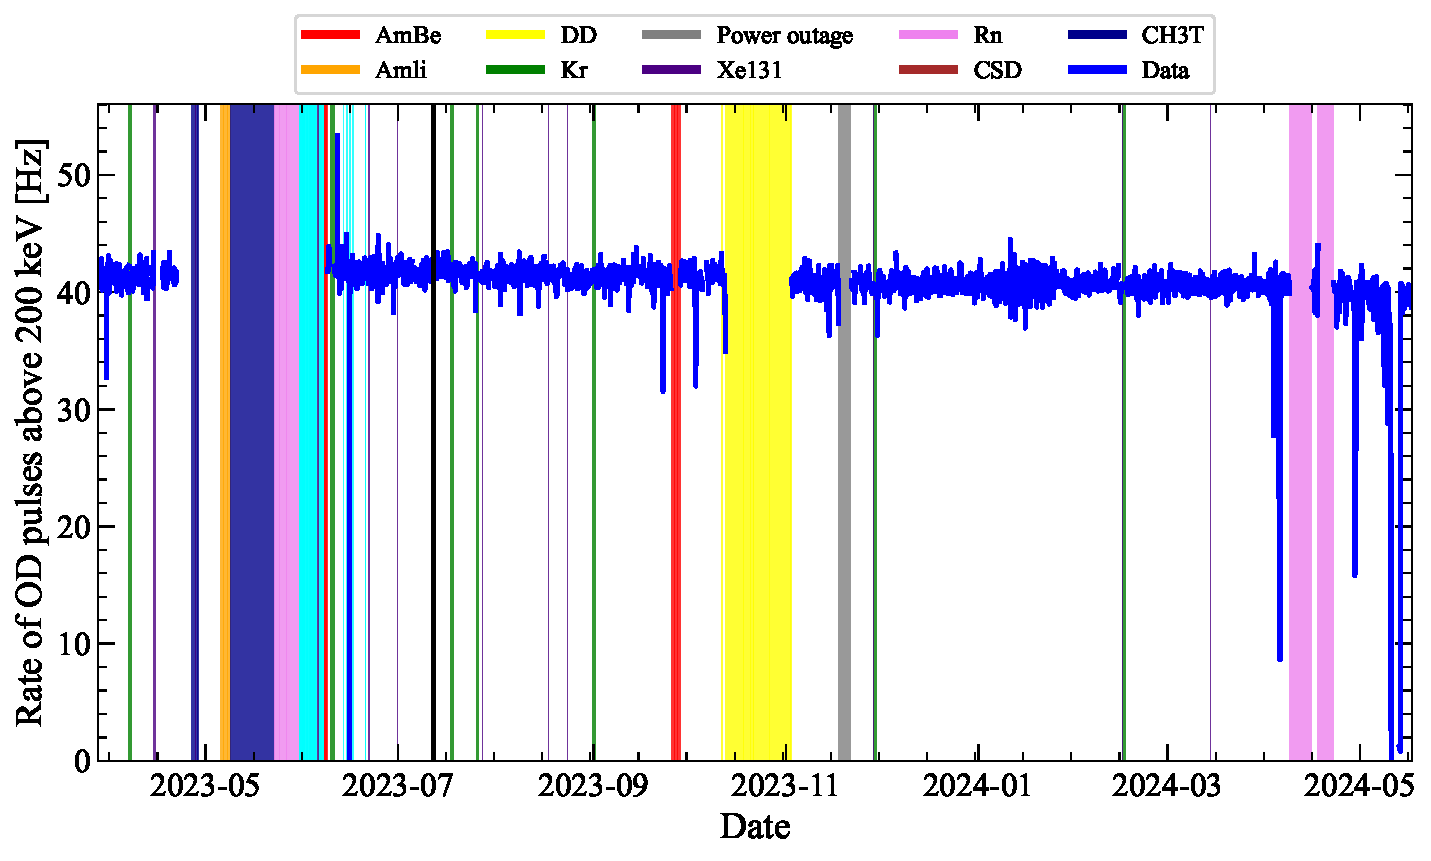
\includegraphics[width=\textwidth]{figures/VetoEfficiency/prem_od_stability.pdf}
	\caption[Rate of OD pulses above 200~keV over the WS2024 science run.]{Rate of OD pulses above 200~keV (as defined by WS2022 energy calibration) over the WS2024 science run. Various periods of calibration are indicated by the coloured regions. The vertical black line indicates the }
	\label{fig:VetoEff/deadtime_stability_prem}
\end{figure}

\section{Neutron veto efficiency}\label{sec:VetoEff/efficiency}
In order to estimate the neutron background of LZ during a science run, we must know what fraction of neutron induced NR single scatters produce a signal in the veto detectors. We call this quantity the \textit{veto efficiency}.
In this section, the efficiency of tagging background neutrons using the Skin and OD detectors is calculated.
This is performed by calculating the efficiency on AmLi and DD calibration data and comparing to simulations.
The difference between efficiencies from simulations and data is then used to calculate an offset factor.
The efficiency is then calculated for detector NR simulations and the observed offset factor is used to estimate the tagging efficiency for events classified as detector NR \cite{LZ:2022ysc,LZ:2024zvo}.
The efficiency is defined as:
\begin{equation}\label{eqn:VetoEff/neutron_tagging_efficiency}
	\eta\;[\%] = \frac{\textrm{N. Events passing TPC analysis cuts + veto cuts}}{\textrm{N. Events passing TPC analysis cuts}} \times 100
\end{equation}
and the inefficiency is defined as $\cancel{\eta}=100-\eta$. For all veto efficiency calculations in this chapter, if a pulse in the Skin or OD passes any of the selections outlined in \autoref{tab:VetoEff/sr3_veto_cuts}, then the event is included in the number of events in the numerator of \autoref{eqn:VetoEff/neutron_tagging_efficiency}. The efficiency based on this decision logic is the \textit{total veto efficiency}.

Two additional efficiencies are investigated: \textit{delayed veto efficiency} defined as events where a pulse is observed that fulfils either of the Skin delayed or OD delayed selection criteria, denoted by $\eta_\text{delayed}$; and \textit{OD-delayed veto efficiency} defined as events where a pulse is observed that fulfils the OD delayed selection criteria, denoted by $\eta_\text{OD-delayed}$.

Unless otherwise stated, all veto efficiencies presented follow the \textit{total veto efficiency} logic.

\subsection{Neutrons from calibration sources}\label{sec:VetoEff/NeutronsFromCalibrationSources}
LZ utilises two neutron sources, AmLi and deuterium-deuterium (DD) neutron generator, to calibrate the detectors response to nuclear recoils and to measure the neutron tagging efficiencies of the veto detectors. The following two sections will detail the veto calculation for each of the calibration data sets.

\subsubsection{AmLi}\label{sec:VetoEff/AmLi_Efficiency}
AmLi sources are a compound of \textsuperscript{241}Am $\alpha$-radioactivity and \textsuperscript{7}Li produce low-energy neutron emission via nuclear $(\alpha,\text{n})$ reactions. Alphas from $^{241}$Am decay bombard the $^{7}$Li nuclei. This leads to a nuclear reaction of type \textsuperscript{7}Li$+\alpha \rightarrow$\textsuperscript{11}B\textsuperscript{*}. The excited \textsuperscript{11}B nucleus then decays to \textsuperscript{11}B via neutron emission. The neutrons produced by the AmLi sources have a maximum energy of $\sim1.5~\text{MeV}$ which results in a nuclear recoils depositing up to $\sim45~\text{keV}_{nr}$ of energy \cite{LZ:2024bsz}. Gamma radiation is also emitted in the \textsuperscript{241}Am decay to various states of \textsuperscript{237}Np and is an associated background to the reaction neutrons. The neutron to gamma ray emission ratio is 0.032 \cite{Sazzad:2023uqs}. The gamma ray background of the AmLi source is accounted for by the accidental correction factors described in \autoref{sec:VetoEff/AmLiAccCorrection}. The characterisation of the LZ AmLi sources is discussed in detail in Ref.~\cite{Sazzad:2023uqs}.

AmLi calibration data used in this study was taken during the May 2023 calibration campaign prior to the WS2024 science run. Events which arre classified as single scatters by LZap and pass the selection outlined in \autoref{tab:VetoEff/amli_efficiency_cuts} are used for the study. Two additional cuts are applied to the calibration data:
\begin{enumerate}
	\item \textit{CSD tube position selection:} A circular cut on the reconstructed position of the SS S1 pulse in the TPC such that events from just one CSD tube are selected at a time. During the calibration campaign, sources were simultaneously deployed in each of the CSD tubes at equal heights (three separate height positions were used, $z=100~\text{mm},700~\text{mm},1300~\text{mm}$ relative to cathode at $z=0~\text{mm}$). Whereas separate simulations were produced with a single source in each CSD tube at three different heights (equal to the $z$-position used in the calibration campaign). 
    The circular cut selects events that have an SS S1 reconstructed position within a 50~mm radius of the CSD tube using the following equation:
    \begin{equation}\label{eqn:VetoEff/CSDSelection}
        \sqrt{(\text{S1}_x-\text{CSD}_x^i)^2+(\text{S1}_y-\text{CSD}_y^i)^2}<50
    \end{equation}
    where S1$_{x,y}$ is the reconstructed $(x,y)$-position of the S1 pulse in the SS and $\text{CSD}_{x,y}^i$ is the $(x,y)$-position of CSD where $i=1,2,3$ for each of the three CSD tubes.
    The boundaries of the cuts for each of the CSD tubes is shown in \autoref{fig:VetoEff/CSDSelection}. 
    \begin{figure}[!ht]
    \centering
        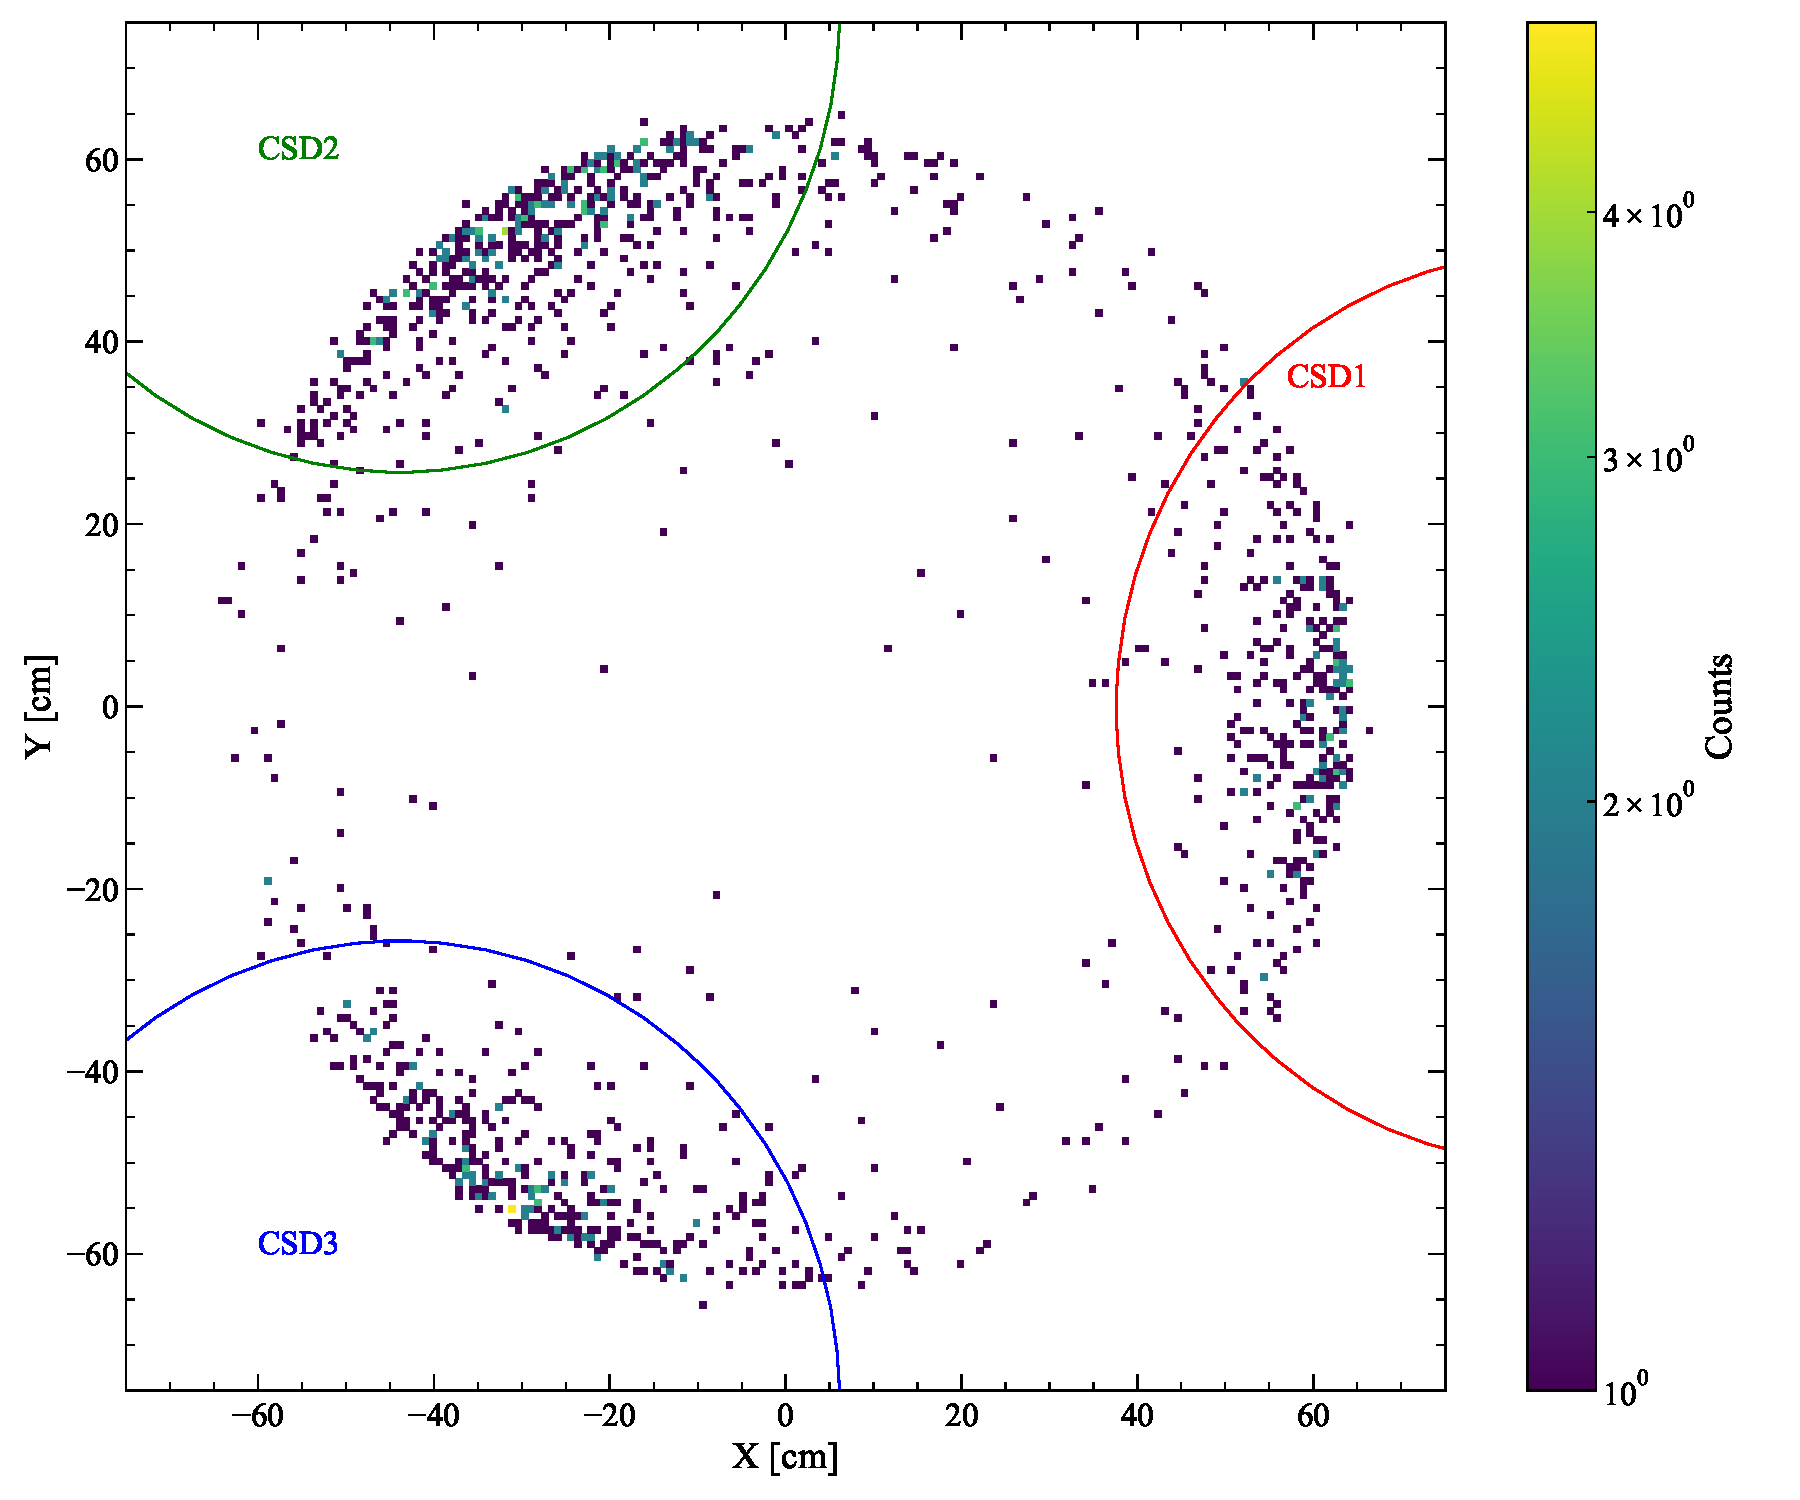
\includegraphics[width=0.7\textwidth]{figures/VetoEfficiency/CircularCSDCut.pdf}
        \caption{X-Y distribution of SS S1 pulses in the TPC for AmLi sources positioned at 700mm. Each of the circular cuts are overlaid on the plot.}
        \label{fig:VetoEff/CSDSelection}
    \end{figure}
    The position dependence of the veto efficiency can be examined by applying the CSD tube selection to data collected at different $z$-positions. The veto efficiency for different CSD tubes and $z$-positions is shown in \autoref{fig:VetoEff/VetoEffPositionDependence}.
    \begin{figure}[!ht]
    	\centering
    	\begin{subfigure}[b]{0.49\textwidth}
    		\centering
    		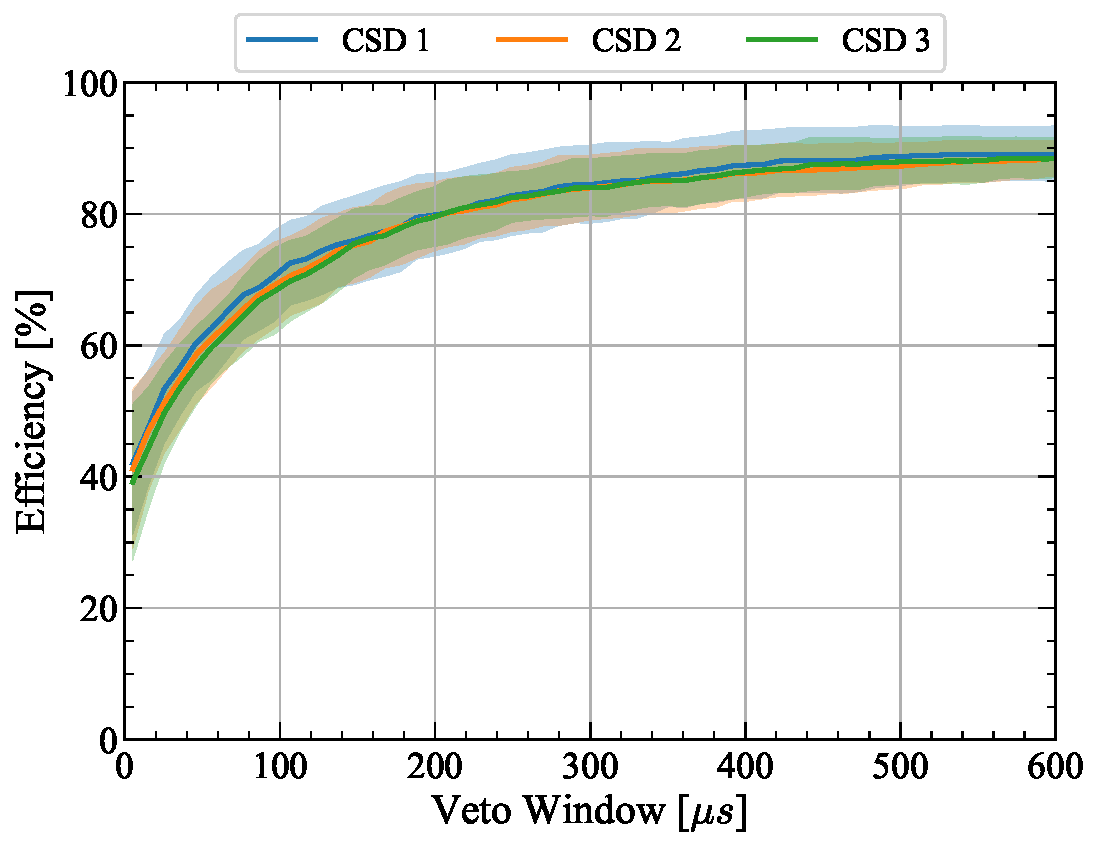
\includegraphics[width=\textwidth]{figures/VetoEfficiency/Eff_AmLi_Total_AllCSD.pdf}
    		\caption{}
            \label{fig:VetoEff/VetoEffPositionDependenceZPos}
    	\end{subfigure}
    	\hfill
    	\begin{subfigure}[b]{0.49\textwidth}
    		\centering
    		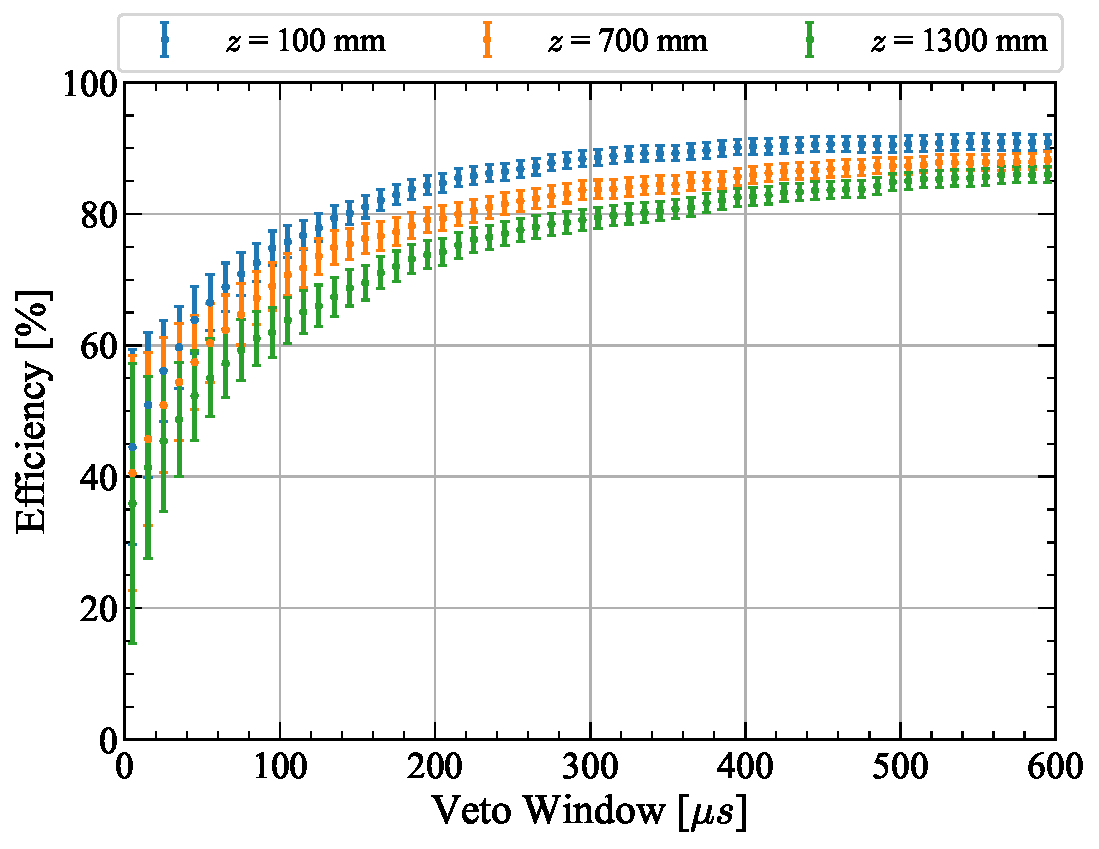
\includegraphics[width=\textwidth]{figures/VetoEfficiency/Eff_AmLi_Total_AllHeights.pdf}
            \caption{}
    		\label{fig:VetoEff/VetoEffPositionDependenceCSD}
    	\end{subfigure}
    	\caption{Position dependent veto efficiencies for different CSD tubes (left) and $z$-positions (right).}
    	\label{fig:VetoEff/VetoEffPositionDependence}
    \end{figure}
	A concern of this cut is that events towards the centre of the TPC are excluded. When the efficiency is averaged across different heights and CSD tube, the average can then be replicated in both data and simulation. 
    The position-averaged efficiency when the CSD cut is applied and without a cut is compatible, at  $(88.21\pm1.03)\%$ and $(88.25\pm1.22)\%$ respectively.
	The cut has $<5\%$ impact across the veto window and $<0.1\%$ impact at the 600~$\mu$s veto window threshold. This comparison is shown in \autoref{fig:VetoEff/CSDSelectionEffComp}.
    \begin{figure}[!ht]
    	\centering
    	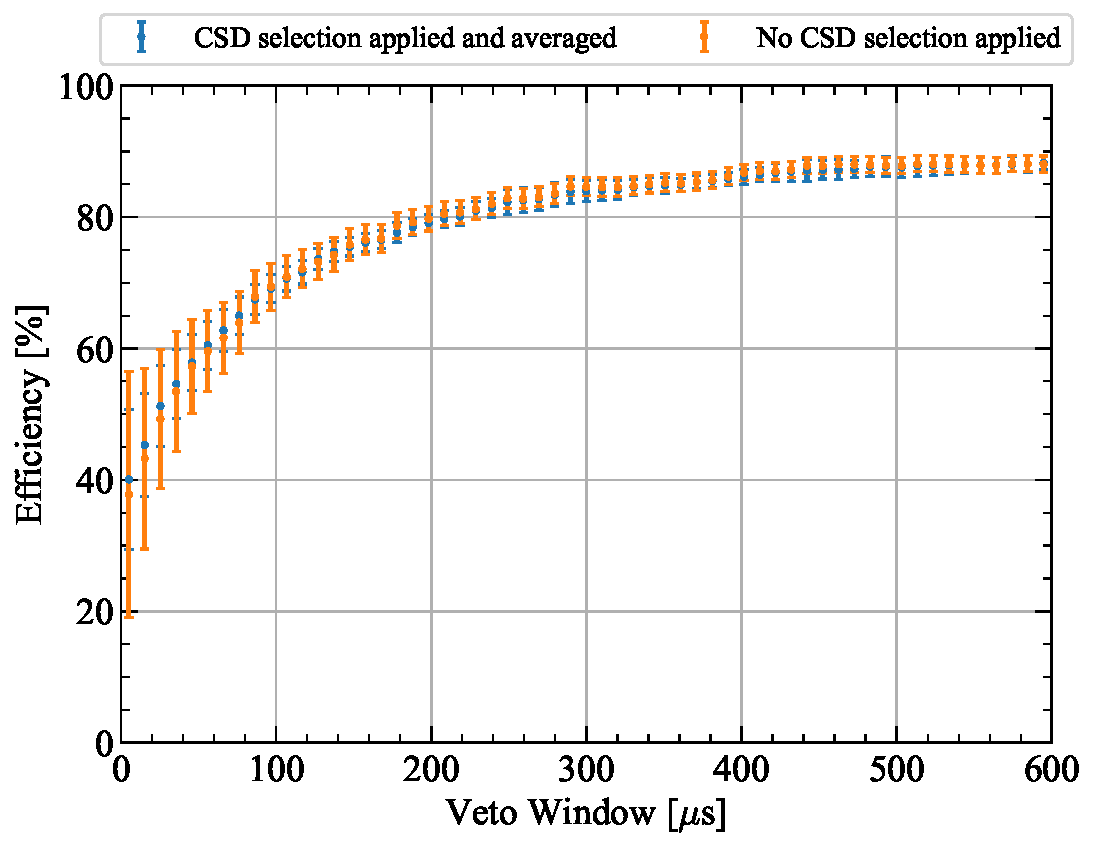
\includegraphics[width=0.7\linewidth]{figures/VetoEfficiency/CSDSelectionCheck.pdf}
    	\caption[CSD tube selection impact on veto efficiency.]{CSD tube selection impact on veto efficiency. The average veto efficiency for events which have a reconstructed position with 50~mm of a CSD tube (blue) is compared to veto efficiency of all events with no CSD selection applied. The cut has $<5\%$ impact across the veto window and $<0.1\%$ impact at the 600~$\mu$s veto window threshold.}
    	\label{fig:VetoEff/CSDSelectionEffComp}
    \end{figure}

	\item \textit{NR-band selection:} SS events which have a S1 and S2 pulse area which lie within 1-$\sigma$ of NR band mean are selected for the veto efficiency calculation.
    The NR bands generated using the Noble Element Simulation Technique (NEST) \cite{NEST2011} are shown in \autoref{fig:VetoEff/SR3NRBands}. 
    The selection is defined as:
    \begin{equation}\label{eqn:VetoEff/NRBandSelection}
        -1<\frac{log_{10}(\text{S2}_\text{obs.})-\overline{log_{10}(\text{S2})}(\text{S1}_\text{obs.})}{\sigma_{log_{10}(\overline{\text{S2}})}(\text{S1}_\text{obs.})}<1
    \end{equation}
    where $\text{S1}_\text{obs.}$ and $log_{10}(\text{S2}_\text{obs.})$ are the observed pulse areas from the SS, $\overline{log_{10}(\text{S2})}(\text{S1}_\text{obs.})$ is the mean S2 corresponding to a observed S1 with $\sigma_{log_{10}(\overline{\text{S2}})}(\text{S1}_\text{obs.})$ based on the NEST model. The purpose of this cut is to improve the purity of the selection and retains 63\% of the data.
    \begin{figure}[!ht]
    \centering
    \begin{subfigure}[b]{0.49\textwidth}
        \centering
        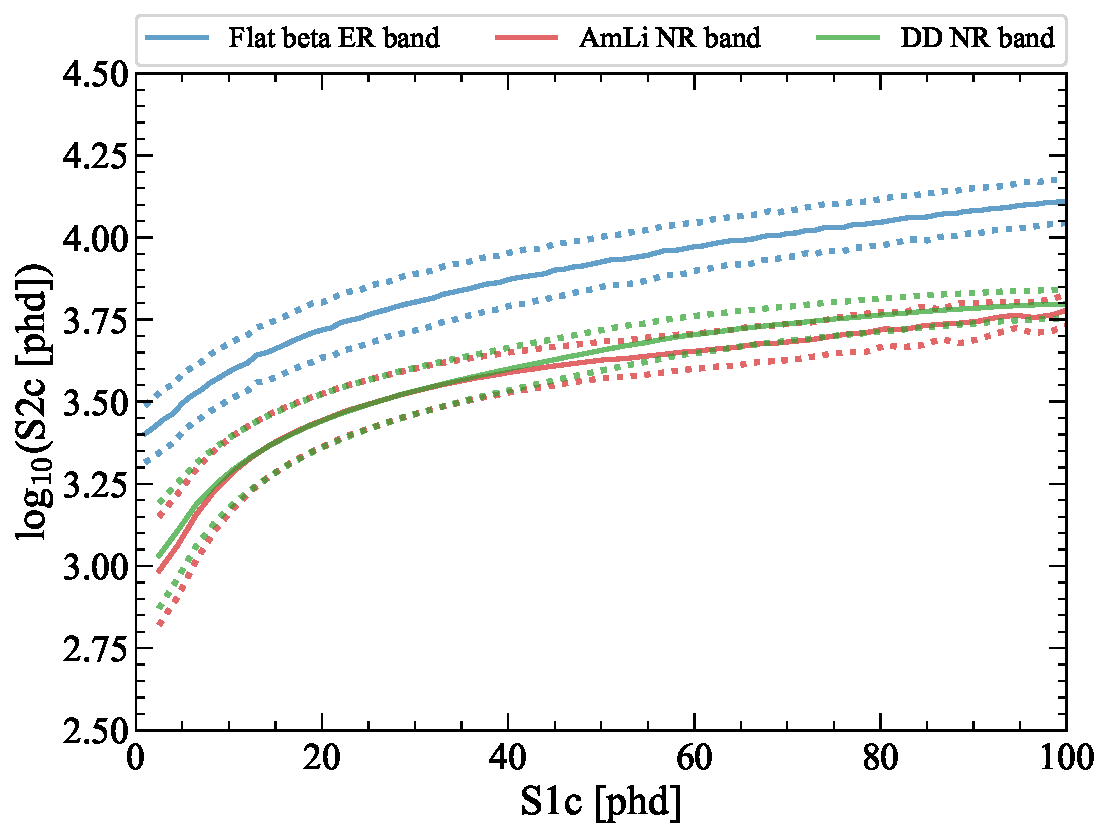
\includegraphics[width=\textwidth]{figures/VetoEfficiency/NRBands.pdf}
        \caption{}
        \label{fig:VetoEff/SR3NRBands}
    \end{subfigure}
    \hfill
    \begin{subfigure}[b]{0.49\textwidth}
        \centering
        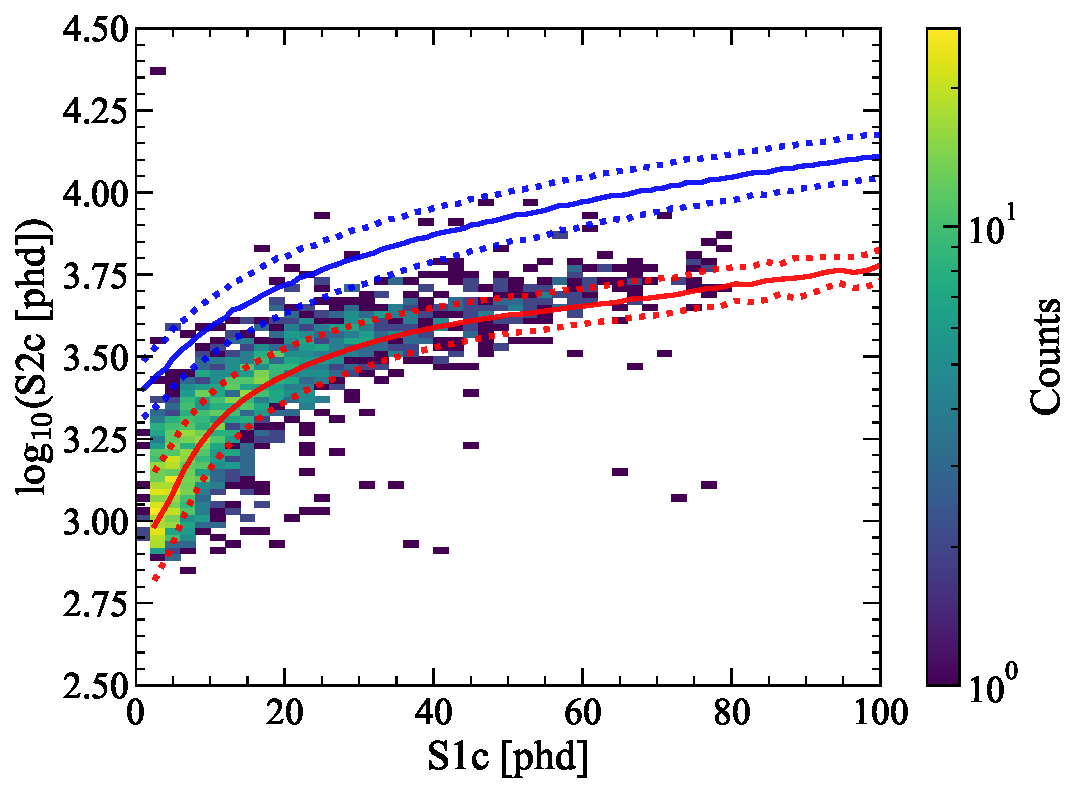
\includegraphics[width=\textwidth]{figures/VetoEfficiency/AmLi700_NRBands.pdf}
        \caption{}
        \label{fig:VetoEff/AmLi700_NRBands}
    \end{subfigure}
    \caption{\textbf{Left:} The NR band means (solid line) with 1-$\sigma$ boundaries (dashed lines) for AmLi and DD calibration sources and a flat beta ER band mean with 1-$\sigma$ boundary. Both NR and ER bands and 1-$\sigma$ boundaries were generated using NEST. \textbf{Right:} AmLi calibration data at $z=700~\text{mm}$ with the corresponding NR band mean and 1-$\sigma$ boundary overlaid.}
    \label{fig:VetoEff/SR3NRBands&AmLi700mmData}
\end{figure}
\end{enumerate}

\subsubsection{Accidental correction factor calculation}\label{sec:VetoEff/AmLiAccCorrection}
If during the calibration, neutrons and gamma rays cause additional veto signals when an unconnected NR event is recorded in the TPC, the veto efficiency will be over estimated. In this chapter, I will call these events \textit{accidental coincidences}\footnote{In LZ, accidental coincidences is also used as a term for spuriously paired S1 and S2 false events but this is not a concern in this chapter.}. To account for this, we estimate the rate of such non-connected vetoes with a sample of events from the calibration dataset randomly triggered in time. Neutrons which are associated with accidental coincidences are produced via additional $(\alpha,\text{n})$ reactions of the AmLi source whilst gamma rays are produced from neutron capture on Gd and H in the GdLS. A small percentage of gamma rays a produced by the $\alpha$ decay of \textsuperscript{241}Am \cite{Sazzad:2023uqs}.

We define the probability of no veto signal in the absence of a TPC interactions as $P(a=0)$, where $a$ is the number of veto detectors observing a pulse. We also define the true veto inefficiency $\cancel\eta_\text{true}$ as the probability, given a TPC interaction, that no veto signal is caused by the neutron that caused \emph{the interaction in the TPC}. Since in $1-P(a=0)$ of cases, such an event will have a spurious veto the observed veto inefficiency will be $\cancel\eta_\text{obs.}=P(a=0)\cdot\cancel\eta_\text{true}$. The observables are the number of TPC SS NR events $N$, the number of those events without a veto signal $M$, the number of randomly triggered `events' $N_\text{random}$, and the number of times a randomly triggered event without a veto signal $M_\text{random}$, giving:
\begin{align}
    \cancel\eta_\text{obs.}&=\frac{M}{N}\\
    P(a=0)&=\frac{M_\text{random}}{N_\text{random}}\\
    \hat{\cancel\eta}&=\frac{\cancel\eta_\text{obs.}}{P(a=0)}\\
    &=\frac{M/N}{M_\text{random}/N_\text{random}},
\end{align}
where $\hat{\cancel\eta}$ is the estimated veto inefficiency for given veto selection. The accidental correction and veto efficiency are correlated with the length of the veto window and veto pulse thresholds. Scans over the entire delayed veto window in 10~$\mu$s steps to observe the change in the correction factor over time is shown in \autoref{fig:VetoEff/SR3AmLi_700mm_Corrections}. The probability of observing zero accidental pulses in the veto detector decreases with increasing veto window size. The probability of observing a coincident neutron from the AmLi or gamma from neutron capture on Gd and H in the GdLS increases with veto window size. At the chosen delayed cut window length of 600~\textmu s, $P_a(0)=0.79\pm0.03$. 
The impact of the accidental correction when applied to the observed efficiency is shown in \autoref{fig:VetoEff/AmLiAccidentalCorrectionImpact}. The impact can be as large at 20\% at large cut windows.

\begin{figure}[!ht]
    \centering
    \begin{subfigure}[b]{0.49\textwidth}
        \centering
        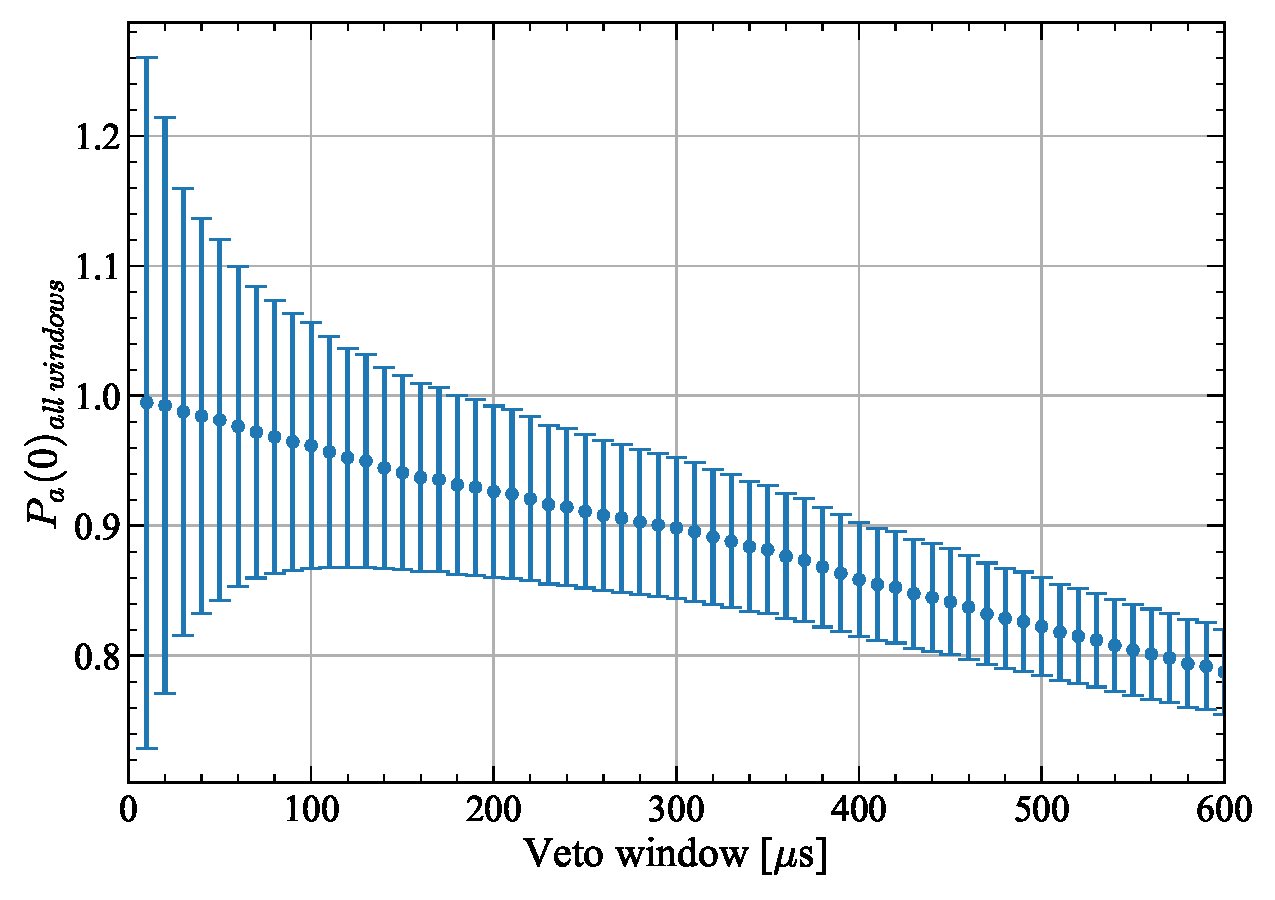
\includegraphics[width=\textwidth]{figures/VetoEfficiency/SR3AmLi_700mm_Corrections_100k.pdf}
        \caption{}
        \label{fig:VetoEff/SR3AmLi_700mm_Corrections}
    \end{subfigure}
    \hfill
    \begin{subfigure}[b]{0.49\textwidth}
        \centering
        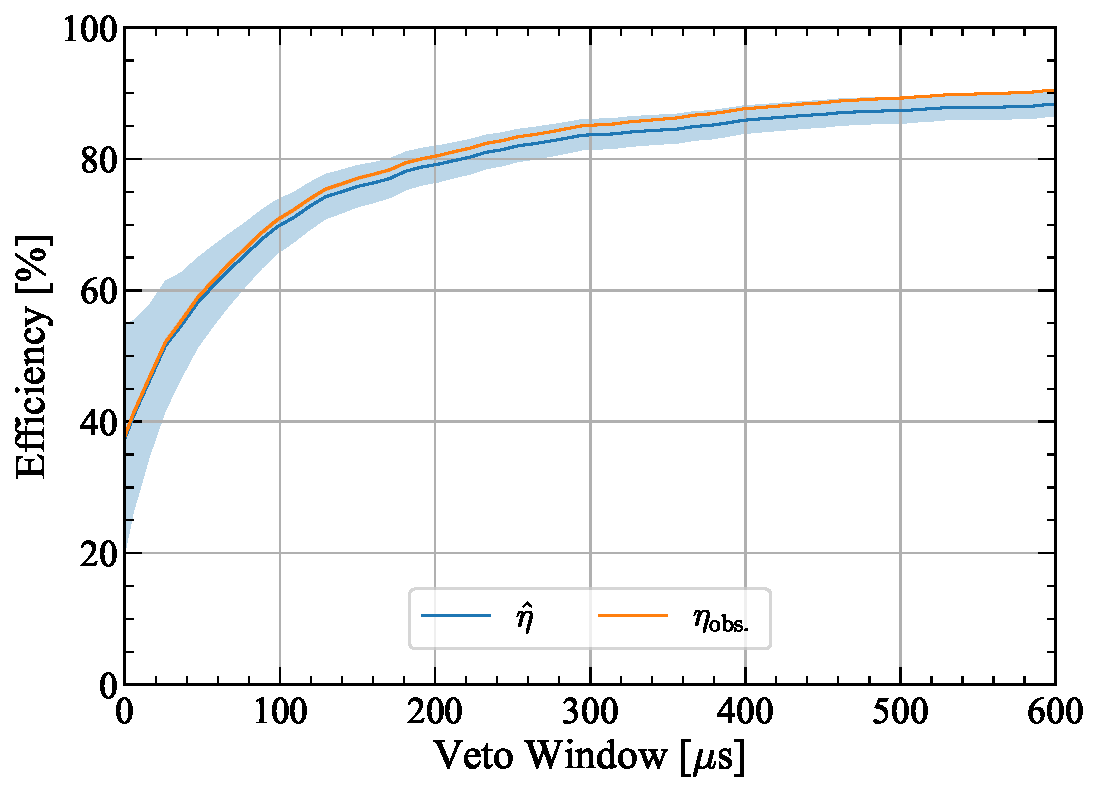
\includegraphics[width=\textwidth]{figures/VetoEfficiency/AmLiAccidentalCheck.pdf}
        \caption{}
        \label{fig:VetoEff/AmLiAccidentalCorrectionImpact}
    \end{subfigure}
    \caption{\textbf{Left:} $P_a(0)$ accidental correction factors over a 600~\textmu s for AmLi calibration sources positioned at $z=700~\text{mm}$. The errors shown are only statistical uncertainties. \textbf{Right:} Comparison between calculated veto efficiencies for AmLi calibration sources positioned at $z=700~\text{mm}$ with accidental correction applied, $\hat{\eta}$, and not applied, $\eta_\text{obs.}$.}
    \label{fig:VetoEff/AmLiAccidentalPlots}
\end{figure}
The final efficiencies measured using AmLi calibration data, corrected for accidental coincidences, and averaged across all positions are shown in \autoref{fig:VetoEff/AmLiEfficiencies}. At the nominal 600~\textmu s veto window, $\eta^\text{Total}_\text{Data}=\big(88.71^{+2.81}_{-2.33}\big)\%$, $\eta^\text{Delayed}_\text{Data}=\big(83.24^{+2.74}_{-2.84}\big)\%$, and $\eta^\text{OD Delayed}_\text{Data}=\big(75.71^{+1.93}_{-2.04}\big)\%$.

\begin{figure}[!ht]
    \centering
    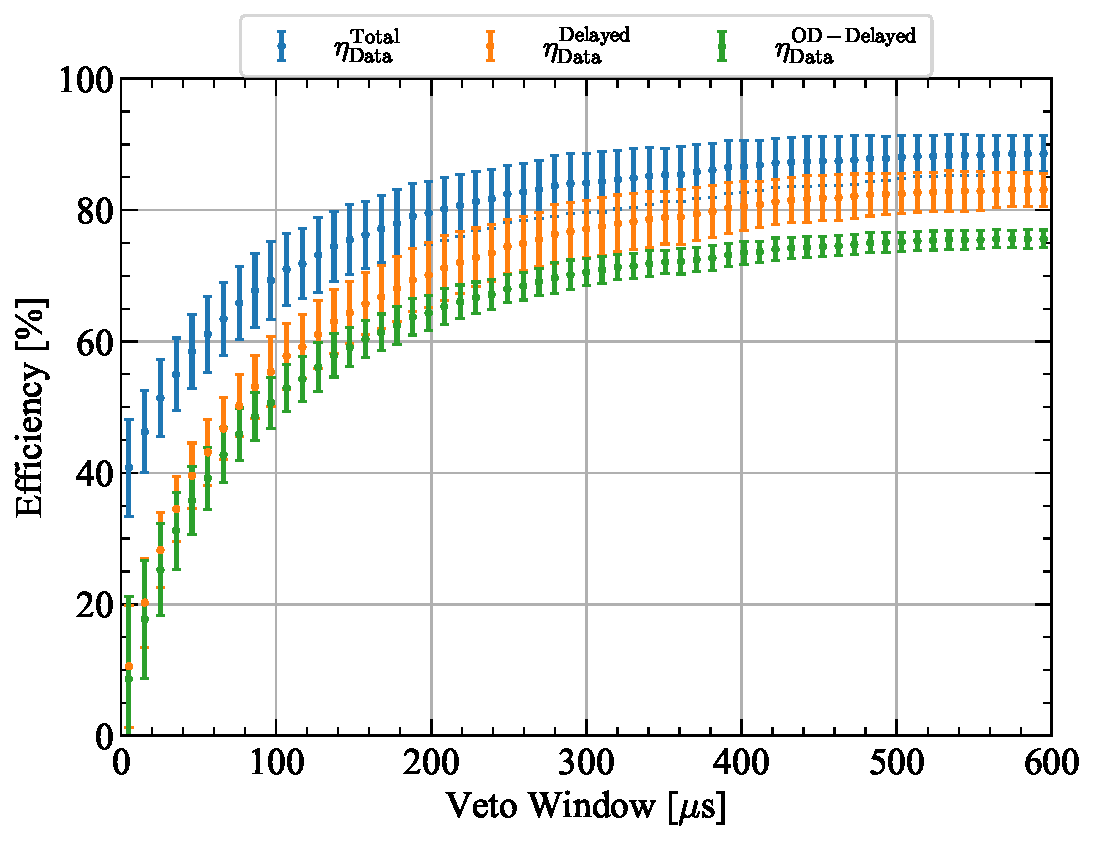
\includegraphics[width=0.7\textwidth]{figures/VetoEfficiency/AmLiEfficiencies_Data.pdf}
    \caption{Final efficiencies measured using AmLi calibration data, corrected for accidental coincidences, and averaged across all positions is shown in \autoref{fig:VetoEff/AmLiEfficiencies}. At 600~\textmu s, $\eta^\text{Total}_\text{Data}=\big(88.71^{+2.81}_{-2.33}\big)\%$, $\eta^\text{Delayed}_\text{Data}=\big(83.24^{+2.74}_{-2.84}\big)\%$, and $\eta^\text{OD Delayed}_\text{Data}=\big(75.71^{+1.93}_{-2.04}\big)\%$.}
    \label{fig:VetoEff/AmLiEfficiencies}
\end{figure}

\subsubsection{Deuterium-deuterium neutron generator}
A deuterium-deuterium (DD) neutron generator is used to produce mono-energetic 2.46~MeV neutrons which result in nuclear recoils depositing up to $74~\text{keV}_{nr}$ of energy. Neutrons are produced by the DD generator as follows: Deuterium is ionized and turned into a plasma by a microwave. Deuterium ions in the plasma are accelerated towards a charged titanium-coated cooper target. D\textsuperscript{+} ions embed into the target form titanium deuteride. Subsequent D\textsuperscript{+} ions fuse to the embed ions and release neutrons via the D+D$\rightarrow$\textsuperscript{3}He+n. The generator is position outside of the water tank and neutrons are collimated and transmitted to the OCV through nitrogen purged conduits \cite{LZ:2024bsz}. The neutron production is pulsed to suppress the ER background rate and enables selection of events coincident with neutron production. Neutron pulsing decreases the impact of accidental coincidences which artificially increases the veto tagging efficiency. Accidental correction factors are still required as pulsing neutron production does not completely suppress accidental coincidences.

DD calibration data used in this study was taken during the October 2023 calibration campaign prior to the WS2024 science run. Events which are classified as single scatters by LZap and pass the selection outlined in \autoref{tab:VetoEff/dd_efficiency_cuts} are used for the study. In addition to these cuts an NR band selection, defined by \autoref{eqn:VetoEff/NRBandSelection}, is applied. It is important to note that DD NR band is different to AmLi NR band. The two different NR bands for the calibration sources are shown in \autoref{fig:VetoEff/SR3NRBands}.

\begin{table}[!ht]
	\centering
	\caption{Outline of cuts applied to DD calibration data for determining the veto efficiency. All cuts are defined in \autoref{sec:app/WSCoreCuts}.}
	\begin{tabular}{lll}
    \hline\hline
	\textbf{Physics cuts}&\textbf{S2 cuts}&\textbf{S1 cuts} \\
	\hline
	Single scatter & S2 width vs drift time & S1 Stinger \\
	S1 threshold & Narrow S2 & S1 TBA vs drift time  \\
	S2 threshold & S2 rise time & S1 HSC cut \\
    Fiducial volume & S2 early peak & S1 Shape \\
	NR Band Selection (defined in \autoref{eqn:VetoEff/NRBandSelection})& S2 XY quality & \\
	& S2 TBA & \\
    \hline\hline
	\end{tabular}
	\label{tab:VetoEff/dd_efficiency_cuts}
\end{table}
The DD calibration data is also corrected for accidental coincidences. The same method is used which is discussed in \autoref{sec:VetoEff/AmLiAccCorrection}. The correction factors used as a function of veto window is shown in \autoref{fig:VetoEff/DDAccCorrectionParameters}. At the nominal 600~\textmu s veto window, $P_a(0)=0.88\pm0.11$. The impact of accidental coincidences on DD data is significantly less than AmLi as events are selected using the trigger from the DD neutron generator. The LZ DAQ is triggered by the generator during neutron production as neutrons are pulsed. The selection of events based on the generator trigger suppresses accidental coincidences. The impact of the accidental corrections on the observed DD veto efficiency is shown in \autoref{fig:VetoEff/DDAccCorrectionImpact_P0}. Due to the high rate of events in the first 60~\textmu s which triggered by the DD neutron generator, the number of randomly triggered events used to generate the accidental correction is zero during this period. Due to the trigger logic used by the LZ DAQ system, randomly triggered events are only allowed if there are no other triggers present. Therefore this period is not considered in the accidental coincidence correction estimate.
\begin{figure}[!ht]
    \centering
    \begin{subfigure}[b]{0.49\textwidth}
        \centering
        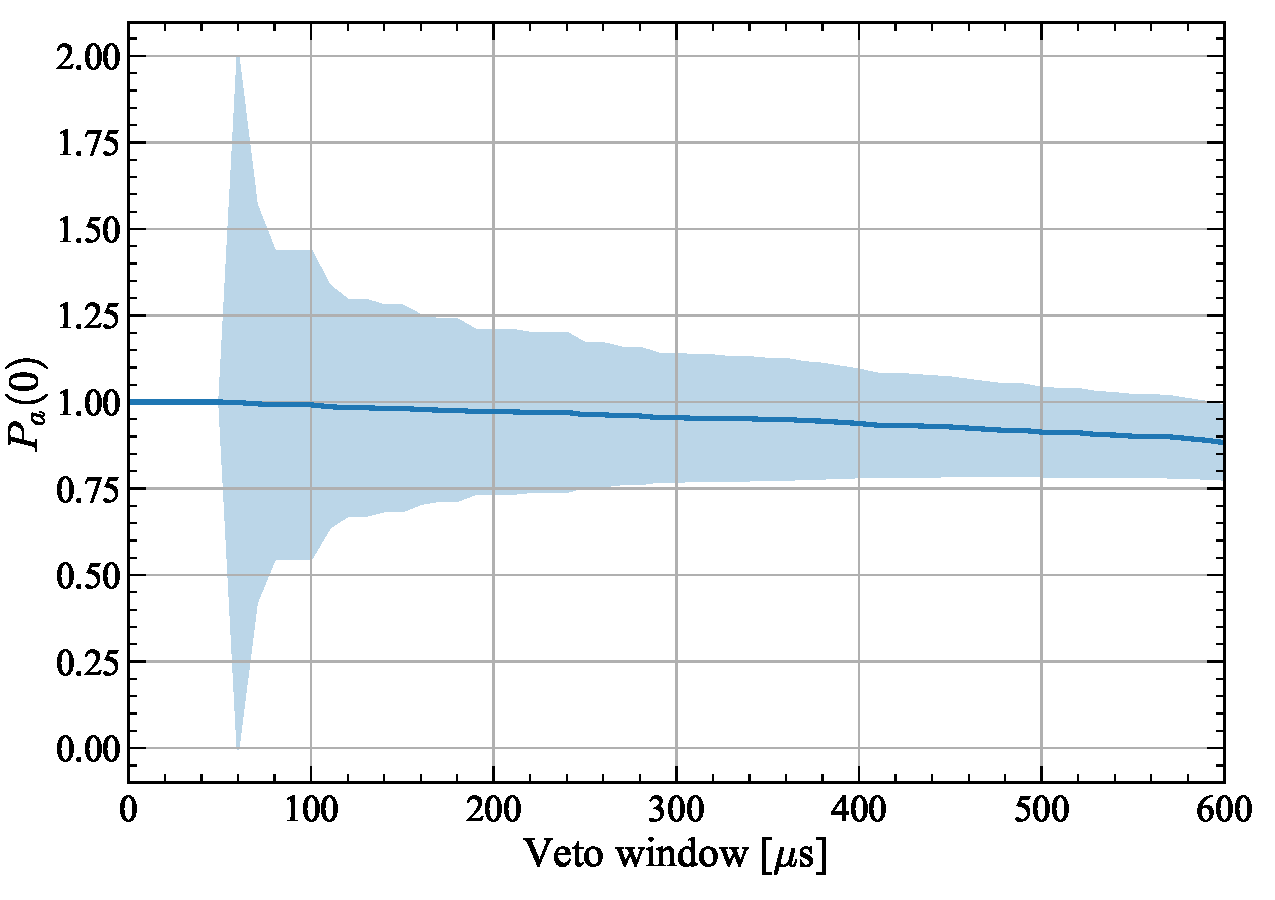
\includegraphics[width=\textwidth]{figures/VetoEfficiency/SR3DDdirect_Corrections_100k.pdf}
        \caption{}
        \label{fig:VetoEff/DDAccCorrectionParameters}
    \end{subfigure}
    \hfill
    \begin{subfigure}[b]{0.49\textwidth}
        \centering
        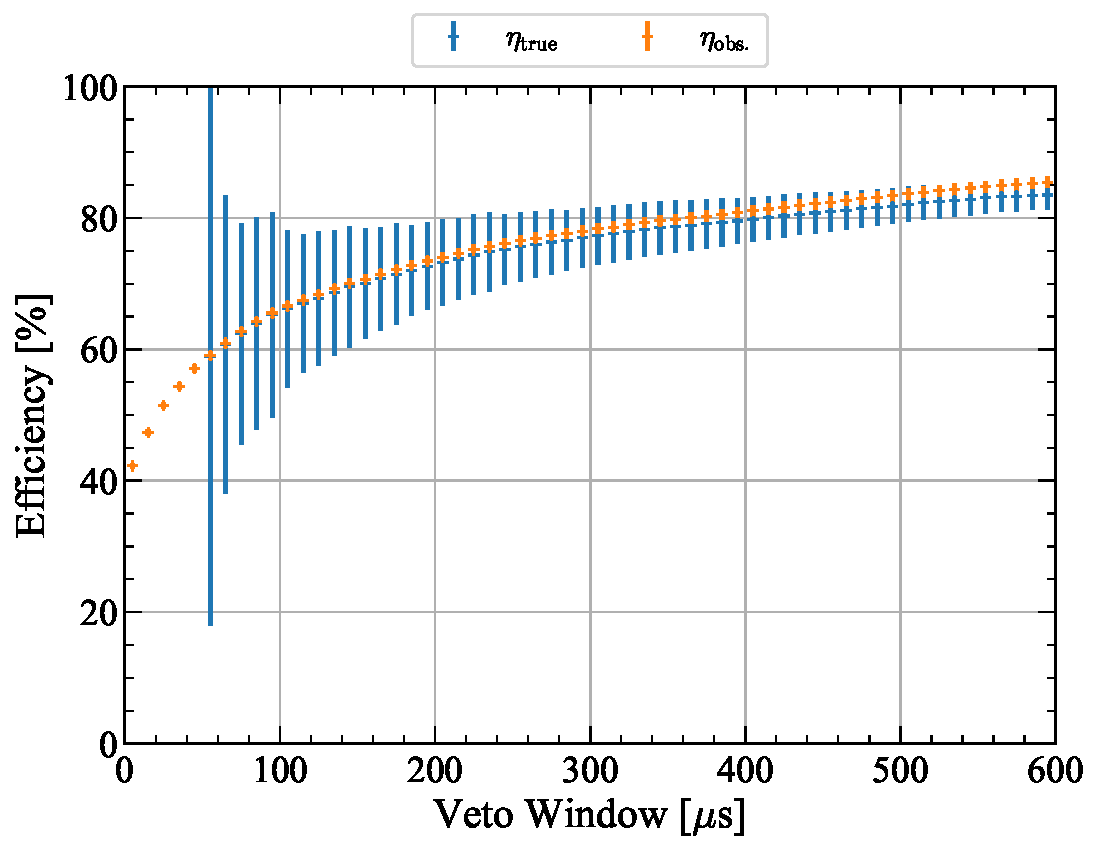
\includegraphics[width=\textwidth]{figures/VetoEfficiency/DDAccidentalCheck.pdf}
        \caption{}
        \label{fig:VetoEff/DDAccCorrectionImpact_P0}
    \end{subfigure}
    \caption{\textbf{Left:} $P_a(0)$ accidental correction factors over a 600~$\mu$s veto window for the DD calibration source data. The errors shown are only statistical uncertainties. The first 60~\textmu s lacks any randomly triggered data to generate accidental corrections during this time. \textbf{Right:} Comparison between calculated veto efficiencies for the DD calibration source with accidental correction applied, $\hat{\eta}$, and not applied, $\eta_\text{obs.}$.}
    \label{fig:VetoEff/DDAccidentalPlots}
\end{figure}

The final efficiencies for DD calibration data corrected for accidental coincidences are shown in \autoref{fig:VetoEff/DDEfficiencies}. At the nominal 600~\textmu s veto window, $\eta^\text{Total}_\text{Data}=\big(87.59^{+1.63}_{-1.64}\big)\%$, $\eta^\text{Delayed}_\text{Data}=\big(83.68^{+2.10}_{-2.09}\big)\%$, and $\eta^\text{OD Delayed}_\text{Data}=\big(81.64^{+2.59}_{-2.58}\big)\%$.

\begin{figure}[ht!]
    \centering
    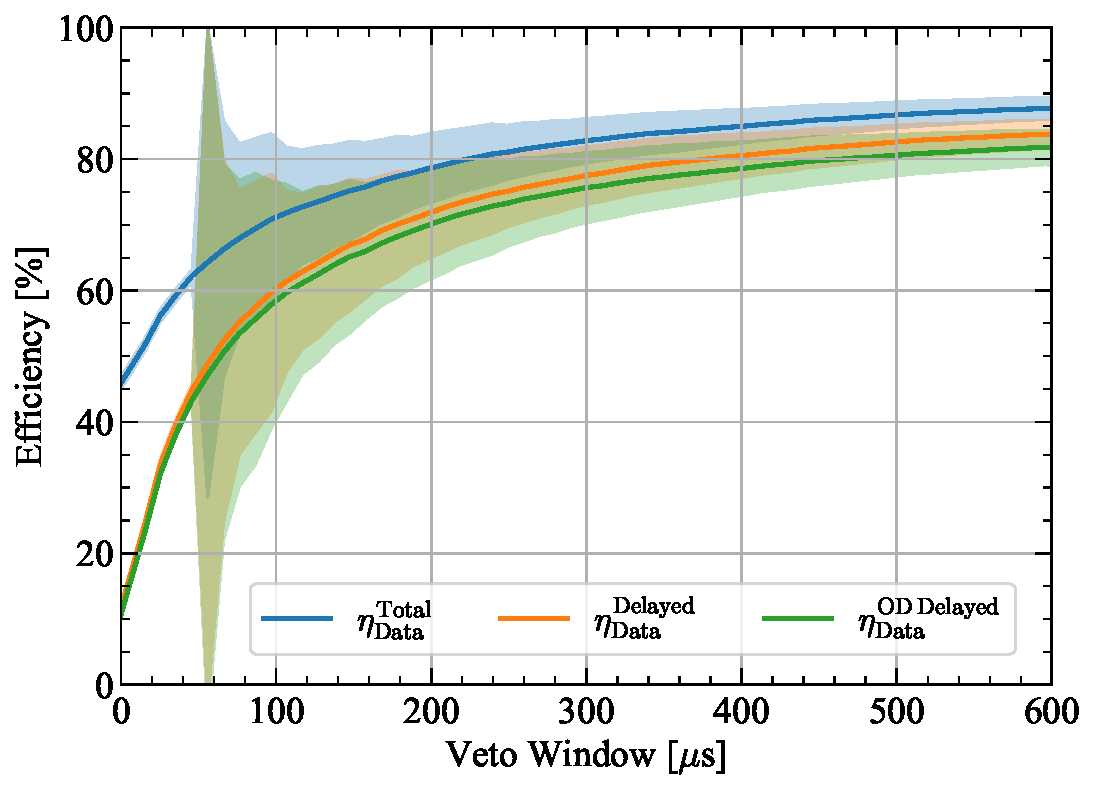
\includegraphics[width=0.7\textwidth]{figures/VetoEfficiency/DDEfficiencies_Data.pdf}
    \caption{DD efficiencies measured in data, all efficiencies are corrected for accidental coincidences. At the nominal 600~\textmu s veto window, $\eta^\text{Total}_\text{Data}=\big(87.59^{+1.63}_{-1.64}\big)\%$, $\eta^\text{Delayed}_\text{Data}=\big(83.68^{+2.10}_{-2.09}\big)\%$, and $\eta^\text{OD Delayed}_\text{Data}=\big(81.64^{+2.59}_{-2.58}\big)\%$.}
    \label{fig:VetoEff/DDEfficiencies}
\end{figure}
\pagebreak
\subsection{Simulated neutrons from calibration sources}
AmLi and DD calibration sources are simulated using LZ's \textit{fast} chain simulation technique (discussed in \autoref{sec:LZ/Simulations}). Simulated events which are classified as single scatters by LZLAMA and pass the following selection: S1 and S2 threshold, fiducial volume, CSD selection (AmLi-only, defined in \autoref{eqn:VetoEff/CSDSelection}), and NR Band Selection (defined in \autoref{eqn:VetoEff/NRBandSelection}) are used to determine the calculated veto efficiency (All cuts are defined in \autoref{sec:app/WSCoreCuts} unless stated otherwise.). 
No accidental gammas or neutrons are present in the simulation, therefore no accidental correction is required. All efficiencies measured using simulated calibration data is presented in \autoref{tab:VetoEff/CalibrationSimulationEfficiencies} and is shown in \autoref{fig:VetoEff/CalibrationSimEfficiencies}.

\begin{figure}[ht!]
    \centering
    \begin{subfigure}[b]{0.49\textwidth}
        \centering
        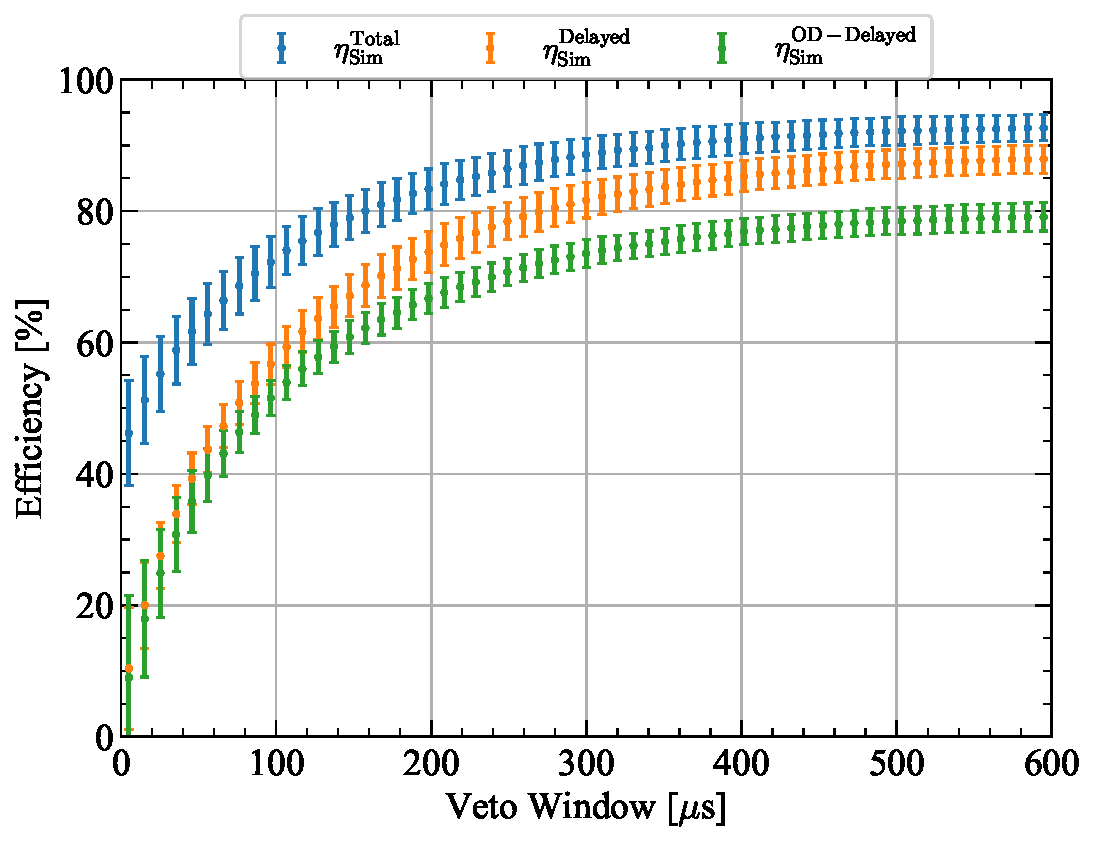
\includegraphics[width=\textwidth]{figures/VetoEfficiency/AmLiEfficiencies_Sim.pdf}
        \caption{}
        \label{fig:VetoEff/AmLiSimEfficiencies}
    \end{subfigure}
    \hfill
    \begin{subfigure}[b]{0.49\textwidth}
        \centering
        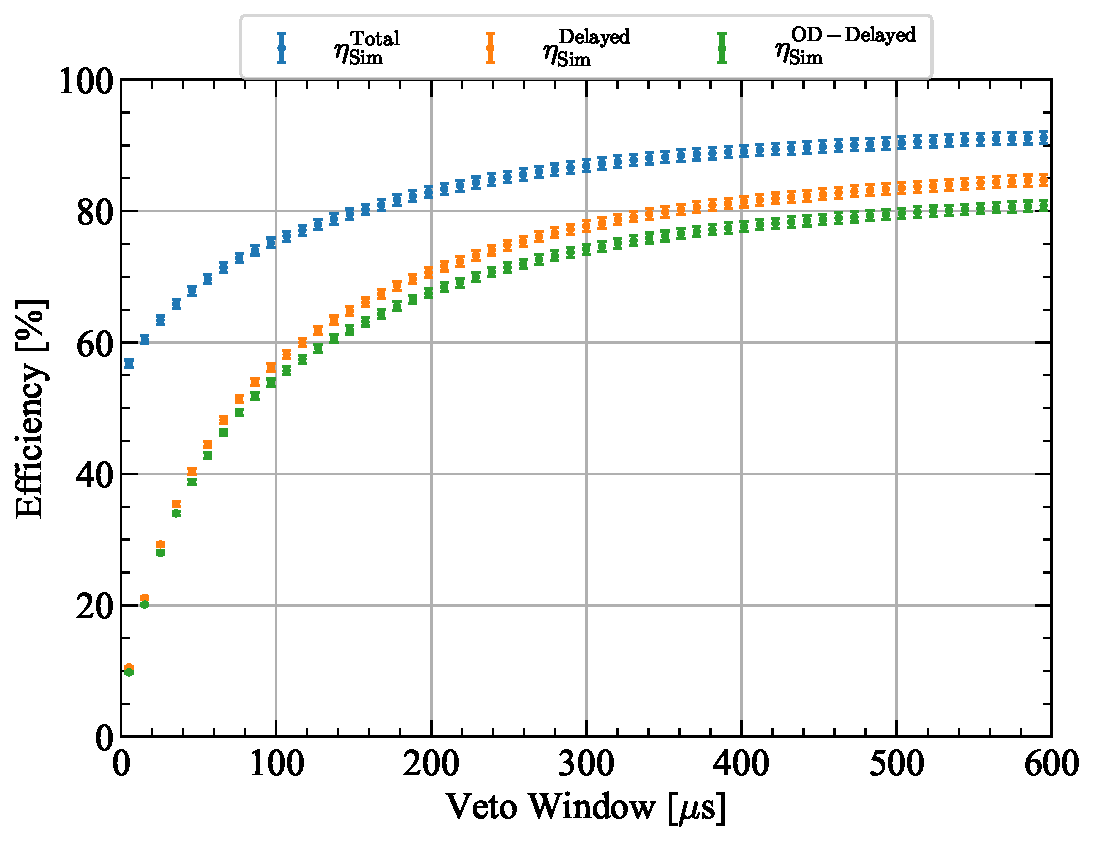
\includegraphics[width=\textwidth]{figures/VetoEfficiency/DDEfficiencies_Sim.pdf}
        \caption{}
        \label{fig:VetoEff/DDSimEfficiencies}
    \end{subfigure}
    \caption{Measured veto efficiencies from AmLi (left) and DD (right) calibration simulations using \textit{Total}, \textit{Delayed}, and \textit{OD Delayed} veto efficiency logic.}
    \label{fig:VetoEff/CalibrationSimEfficiencies}
\end{figure}
\renewcommand{\arraystretch}{1.5}
\begin{table}[h!]
    \centering
    \caption{Estimated efficiencies from AmLi and DD calibration simulations at the nominal 600~\textmu s window.}
    \begin{tabular}{llll}
    \hline\hline
    \textbf{Source} & \textbf{$\eta^\text{Total}_\text{Sim}$ [\%]} & \textbf{$\eta^\text{Delayed}_\text{Sim}$ [\%]} & \textbf{$\eta^\text{OD Delayed}_\text{Sim}$ [\%]}\\
    \hline
    AmLi & $92.68^{+2.32}_{-2.21}$ & $87.90^{+2.53}_{-2.43}$ & $79.12^{+2.63}_{-2.55}$ \\
    DD & $91.20^{+0.92}_{-0.91}$ & $84.77^{+0.85}_{-0.84}$ & $80.85^{+0.81}_{-0.80}$\\
    \hline\hline
    \end{tabular}
    \label{tab:VetoEff/CalibrationSimulationEfficiencies}
\end{table}
\renewcommand{\arraystretch}{1}

The comparison between veto efficiencies calculated for data and simulation for both sources is shown in \autoref{fig:VetoEff/Sim2DataVetoEffComparisons}. The veto efficiency for AmLi is averaged across all CSD positions and $z$-positions. The percentage difference between the calculated veto efficiency is presented below the veto efficiency curves for both sources. Both sources show good agreement when total veto efficiencies are compared with $4.37\%$ and $2.39\%$ difference between data and simulation for AmLi and DD calibration sources respectively.

\iffalse
\begin{table}[!ht]
	\centering
	\caption{Outline of cuts applied to simulation data for determining the veto efficiency. All cuts are defined in \autoref{sec:app/WSCoreCuts} unless stated otherwise.}
	\begin{tabular}{l}
        \hline\hline
        \textbf{Physics cuts}\\
        \hline
        Single scatter\\
        S1 and S2 threshold\\
        Fiducial Volume\\
        CSD Selection (AmLi only, defined in \autoref{eqn:VetoEff/CSDSelection})\\
        NR Band Selection (defined in \autoref{eqn:VetoEff/NRBandSelection})\\
        \hline\hline
	\end{tabular}
	\label{tab:VetoEff/calibration_simulation_efficiency_cuts}
\end{table}
\fi
\begin{figure}[h!]
    \centering
    \begin{subfigure}[b]{0.49\textwidth}
        \centering
        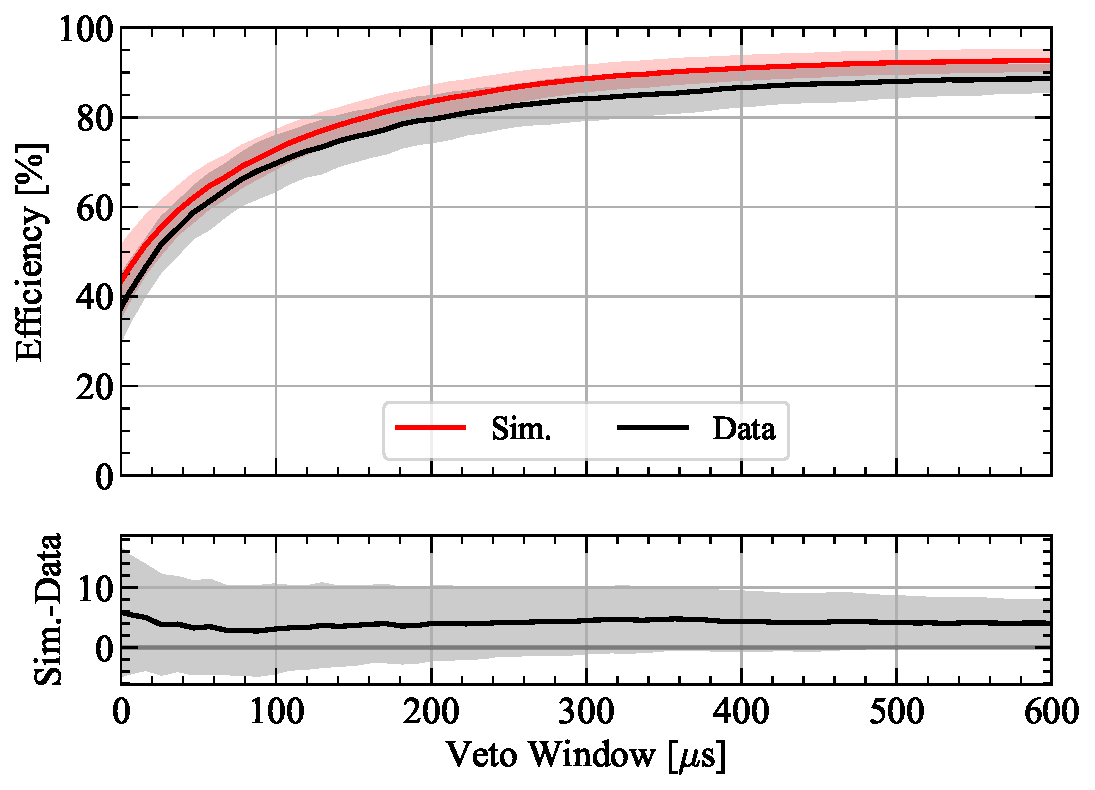
\includegraphics[width=\textwidth]{figures/VetoEfficiency/AmLi_Total_Avg_Ratio.pdf}
        \caption{}
        \label{fig:VetoEff/Sim2DataVetoEffComparisons_AmLi}
    \end{subfigure}
    \hfill
    \begin{subfigure}[b]{0.49\textwidth}
        \centering
        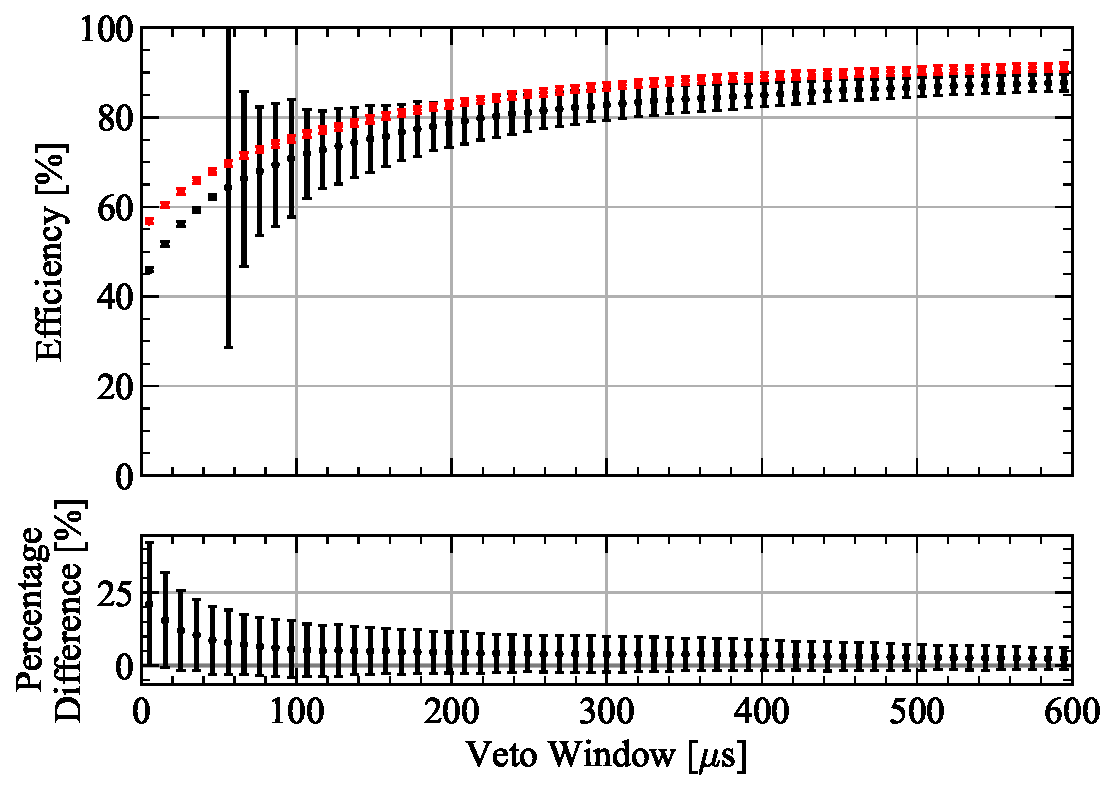
\includegraphics[width=\textwidth]{figures/VetoEfficiency/DDDirect_Total_Ratio.pdf}
        \caption{}
        \label{fig:VetoEff/Sim2DataVetoEffComparisons_DD}
    \end{subfigure}
    \caption{Comparison of calculated data (black) and simulation (red) veto efficiencies for AmLi (left) and DD (right) calibration sources. The difference between the calculated veto efficiency is presented below the veto efficiency curves for both sources. Both sources show good agreement when veto efficiencies are compared with $4.37\%$ and $2.39\%$ difference between data and simulation for AmLi and DD calibration sources respectively. The lower panel of the DD efficiency comparison has been magnified to better present the difference at 600~\textmu s.}
    \label{fig:VetoEff/Sim2DataVetoEffComparisons}
\end{figure}

\subsection{Background neutrons}\label{sec:VetoEff/BackgroundNeutrons}
Detector NR simulations are produced using LZ's \textit{fast} chain simulation technique as part of the official LZ production prior to the WS2024 science run.
As part of this production each of the 644 components which have a radioactive background are simulated.
Simulated events which are classified as single scatters by LZLAMA and pass the following selection cut: S1 and S2 threshold, fiducial volume, were used to determine the calculated veto efficiency (All cuts are defined in \autoref{sec:app/WSCoreCuts}).
The efficiency of tagging neutrons from Uranium Spontaneous Fission (USF) and ($\alpha$,n) events are shown in \autoref{fig:VetoEff/detector_nr_efficiency}. Also shown is the total efficiency.

\iffalse
\begin{table}[!ht]
	\centering
	\caption{Outline of cuts applied to detector NR simulations for determining the veto efficiency. All cuts are defined in \autoref{sec:app/WSCoreCuts}.}
	\begin{tabular}{l}
    \hline\hline
		\textbf{Physics cuts}\\
		\hline
		Single scatter\\
		S1 and S2 threshold\\
		Fiducial Volume\\
        \hline\hline
	\end{tabular}
	\label{tab:VetoEff/detector_nr_simulation_efficiency_cuts}
\end{table}
\fi

\begin{figure}[!ht]
	\centering
	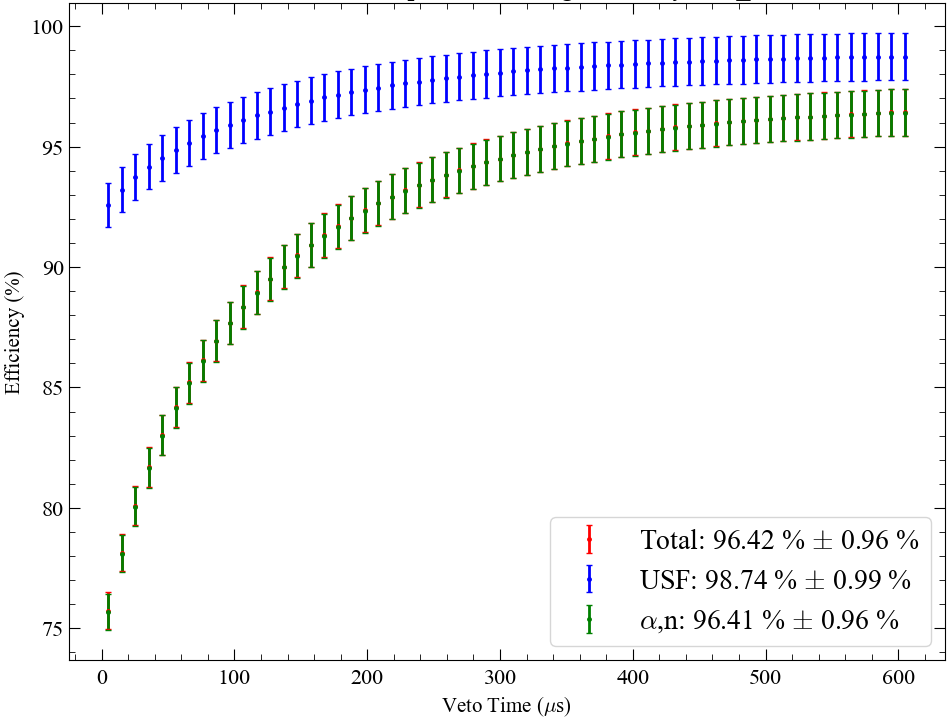
\includegraphics[width=0.7\textwidth]{figures/VetoEfficiency/det_nr_efficiency.png}
	\caption{Efficiencies to veto simulated events which include a single scatter NR TPC. Each of the 644 background component contributions are weighted according to their contribution to the total NR background. TPC NR events are required to have a reconstructed $z$-position corresponding to an average drift time $t_\text{drift}$ between 350~\textmu s and 700~\textmu s in this example.}
	\label{fig:VetoEff/detector_nr_efficiency}
\end{figure}

\subsection{Background neutron efficiency from data}\label{sec:VetoEff/BkgNeutronEff}
The neutron veto efficiency from each calibration source from data and simulation is shown in \autoref{fig:VetoEff/efficiency_summary}. Also shown is the efficiency from simulated background neutrons.
The $z$-position of each point is calculated from the mean drift time, $\overline{t}_{\text{drift}}$, of events which pass the selection outlined in \autoref{sec:VetoEff/BackgroundNeutrons}.
For the detector NR simulations, the events are separated into three $z$-sections by the following criteria:
\begin{itemize}
    \item \textit{Top:} 71~\textmu s $\leq\overline{t}_{\text{drift}}\leq$350~\textmu s
    \item \textit{Middle:} 350~\textmu s $<\overline{t}_{\text{drift}}\leq$700~\textmu s
    \item \textit{Bottom:} 700~\textmu s $<\overline{t}_{\text{drift}}\leq$1030~\textmu s
\end{itemize}

\begin{figure}[!ht]
	\centering
	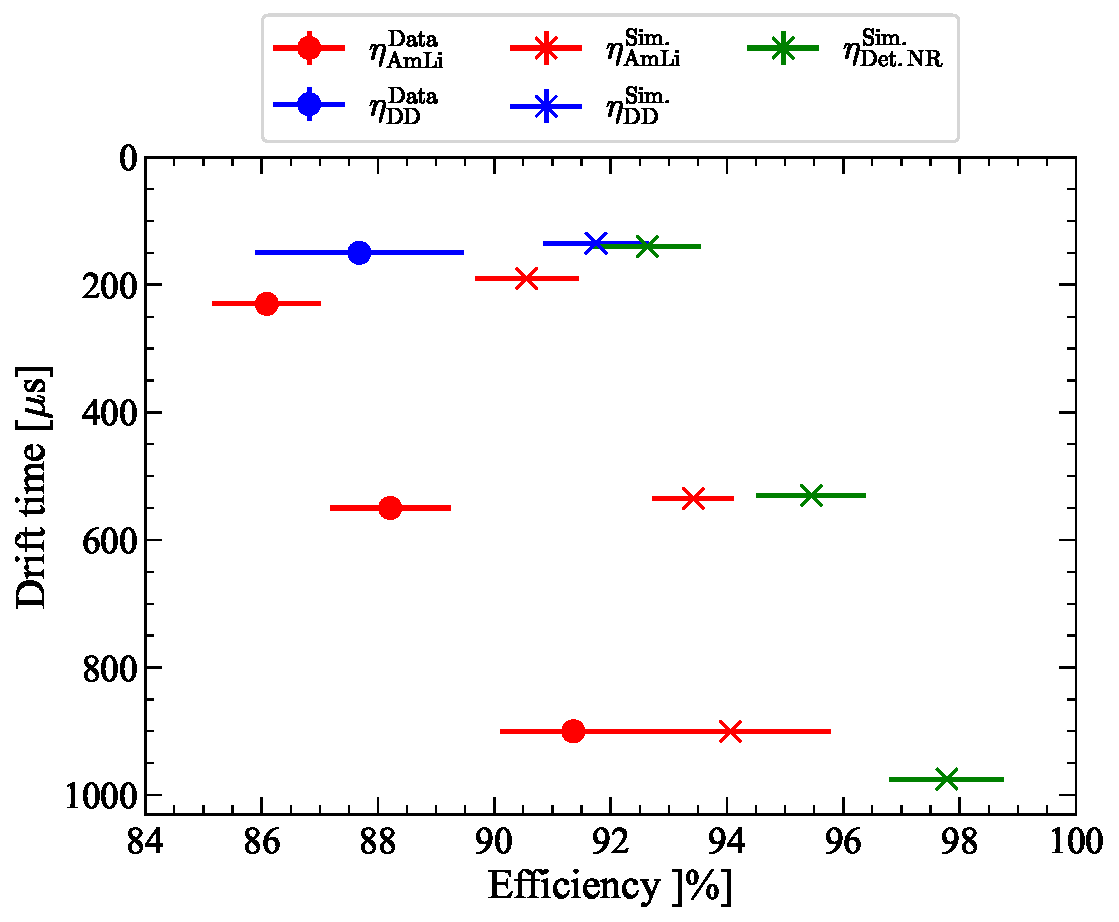
\includegraphics[width=0.7\textwidth]{figures/VetoEfficiency/SummaryPlot.pdf}
	\caption{Summary of efficiency from all simulations and calibration sources.
		The CSD sources are averaged at each deployment position, $z=100~\text{mm},700~\text{mm},1300~\text{mm}$.
		Circle markers represent calculated veto efficiencies from data.
		Star markers represent calculated veto efficiencies from simulation.}
	\label{fig:VetoEff/efficiency_summary}
\end{figure}
$t_{\text{drift}}$ splitting of detector NR simulation is performed to compare the calculated veto efficiencies of the detector NR simulations to veto efficiencies calculated from calibration sources. However, this was not used in the final efficiency evaluation. Shown in \autoref{tab:VetoEff/final_veto_efficiency} are the veto efficiencies of all calibration sources for both simulations and data alongside the veto efficiencies for the detector NR sources.

The importance of this chapter lies in determining LZ's efficiency to reject background neutrons, the estimated veto efficiency for detector NR events, $\eta_{\text{Det. NR}}^{\text{Data}}$. The method to estimate this efficiency is as follows. 
The average simulation calibration efficiency is taken between, $\overline{\eta}_{\text{AmLi}}^{\text{Sim.}}=(92.8\pm2.0)\%$ and $\eta_{\text{DD}}^{\text{Sim.}}=(91.8\pm1.0)\%$ which results in an average efficiency of $\overline{\eta}_{\text{Cal.}}^{\text{Sim.}}=(92.3\pm1.1)\%$.
The average data calibration efficiency is taken between, $\overline{\eta}_{\text{AmLi}}^{\text{Data}}=(88.6\pm2.7)\%$ and $\eta_{\text{DD}}^{\text{Data}}=(91.8\pm1.0)\%$, which results in an average efficiency of $\overline{\eta}_{\text{Cal.}}^{\text{Data}}=(88.2\pm1.6)\%$.
The difference, $\Lambda$, between the simulation calibration and data calibration efficiencies is used as a systematic uncertainty on the efficiency of detector NR simulations.
This process is expressed in \autoref{eqn:VetoEff/DetNR_efficiency}, and produces an estimated veto efficiency for detector NR of $\eta_{\text{Det. NR}}^\text{Data}=(92.2\pm4.3)\%$.
The final uncertainty of the estimated detector NR veto efficiency, $\sigma^\text{Data}_\text{Det. NR}$, is the product of the statistical uncertainty from the simulations $\sigma^\text{Sim.}_\text{Det. NR}=1\%$, and $\Delta=4.2\%$ from the subtraction of the data calibration efficiency from the simulation calibration efficiency. {\color{red}Rewrite this without percentages}
\begin{equation}
    \label{eqn:VetoEff/DetNR_efficiency}
    \begin{split}
    	\overline{\eta}_{\text{Cal.}}^{\text{Sim.}} & = \frac{\overline{\eta}_{\text{AmLi}}^{\text{Sim.}}+\eta_{\text{DD}}^{\text{Sim.}}}{2}\\
    	\overline{\eta}_{\text{Cal.}}^{\text{Data}} & = \frac{\overline{\eta}_{\text{AmLi}}^{\text{Data}}+\eta_{\text{DD}}^{\text{Data}}}{2} \\
    	\Lambda &= \overline{\eta}_{\text{Cal.}}^{\text{Sim.}} - \overline{\eta}_{\text{Cal.}}^{\text{Data}}\\
    	\eta_\text{Det. NR}^\text{Data}   & = \eta_\text{Det. NR}^\text{Sim.} - \Lambda
    \end{split}
\end{equation}
For the 2024 WIMP search result \cite{LZCollaboration:2024lux}, LZ achieved an estimated neutron tagging efficiency, $\eta_\text{Det. NR}^\text{Data}=(92\pm4)\%$.

\begin{table}[!h]
	\centering
	\caption[Summary of veto tagging efficiencies.]{Summary of veto tagging efficiencies.}
	\begin{tabular}{lll}
    \hline\hline
    \textbf{Source}& \textbf{$\eta^\text{Sim.}$ [\%]}& \textbf{$\eta^\text{Data}$ [\%]}\\ 
    \hline
    AmLi (average) & 92.8$\pm$2.0 & 88.6$\pm$2.7\\
    DD & 91.8$\pm$1.0 & 87.7$\pm$1.8\\
    Detector NR & 96.4$\pm$1.0 & 92.2$\pm$4.3\\
    \hline\hline
	\end{tabular}
	\label{tab:VetoEff/final_veto_efficiency}
\end{table}

\section{Veto selection and the 2024 WIMP search result}\label{sec:VetoEff4WIMPSearch}
Candidate events for the WIMP search analysis (see \autoref{chap:WS2024Result}) are selected using a series of event and data selections. The cuts described in the \autoref{sec:VetoEff/VetoSelectionOptimisation} are the ``veto coincidence cuts'' which are used to reject SS events which are accompanied by a coincident signal in the Skin and/or OD. The greatest benefit of the veto system to the WIMP search analysis is the increase in the fiducial volume of the TPC. Background events produced near the walls of the TPC are tagged by the veto system and are rejected from the the analysis. In the absence of the veto system, the optimum method of removing background events near the wall would be to remove that portion of the target mass entirely. This method would result in a 40\% decrease in exposure \cite{lkorley:thesis}. This is not a suitable method for a dark matter direct detection search where the amount of target mass should be maximized where possible. The reconstructed TPC position of events selected by the veto coincidence cuts is shown in \autoref{fig:VetoEff/WS2024_TPCPosPlots_2panel} alongside candidate events used for the 2024 WIMP search analysis.
\begin{figure}[ht!]
    \centering
    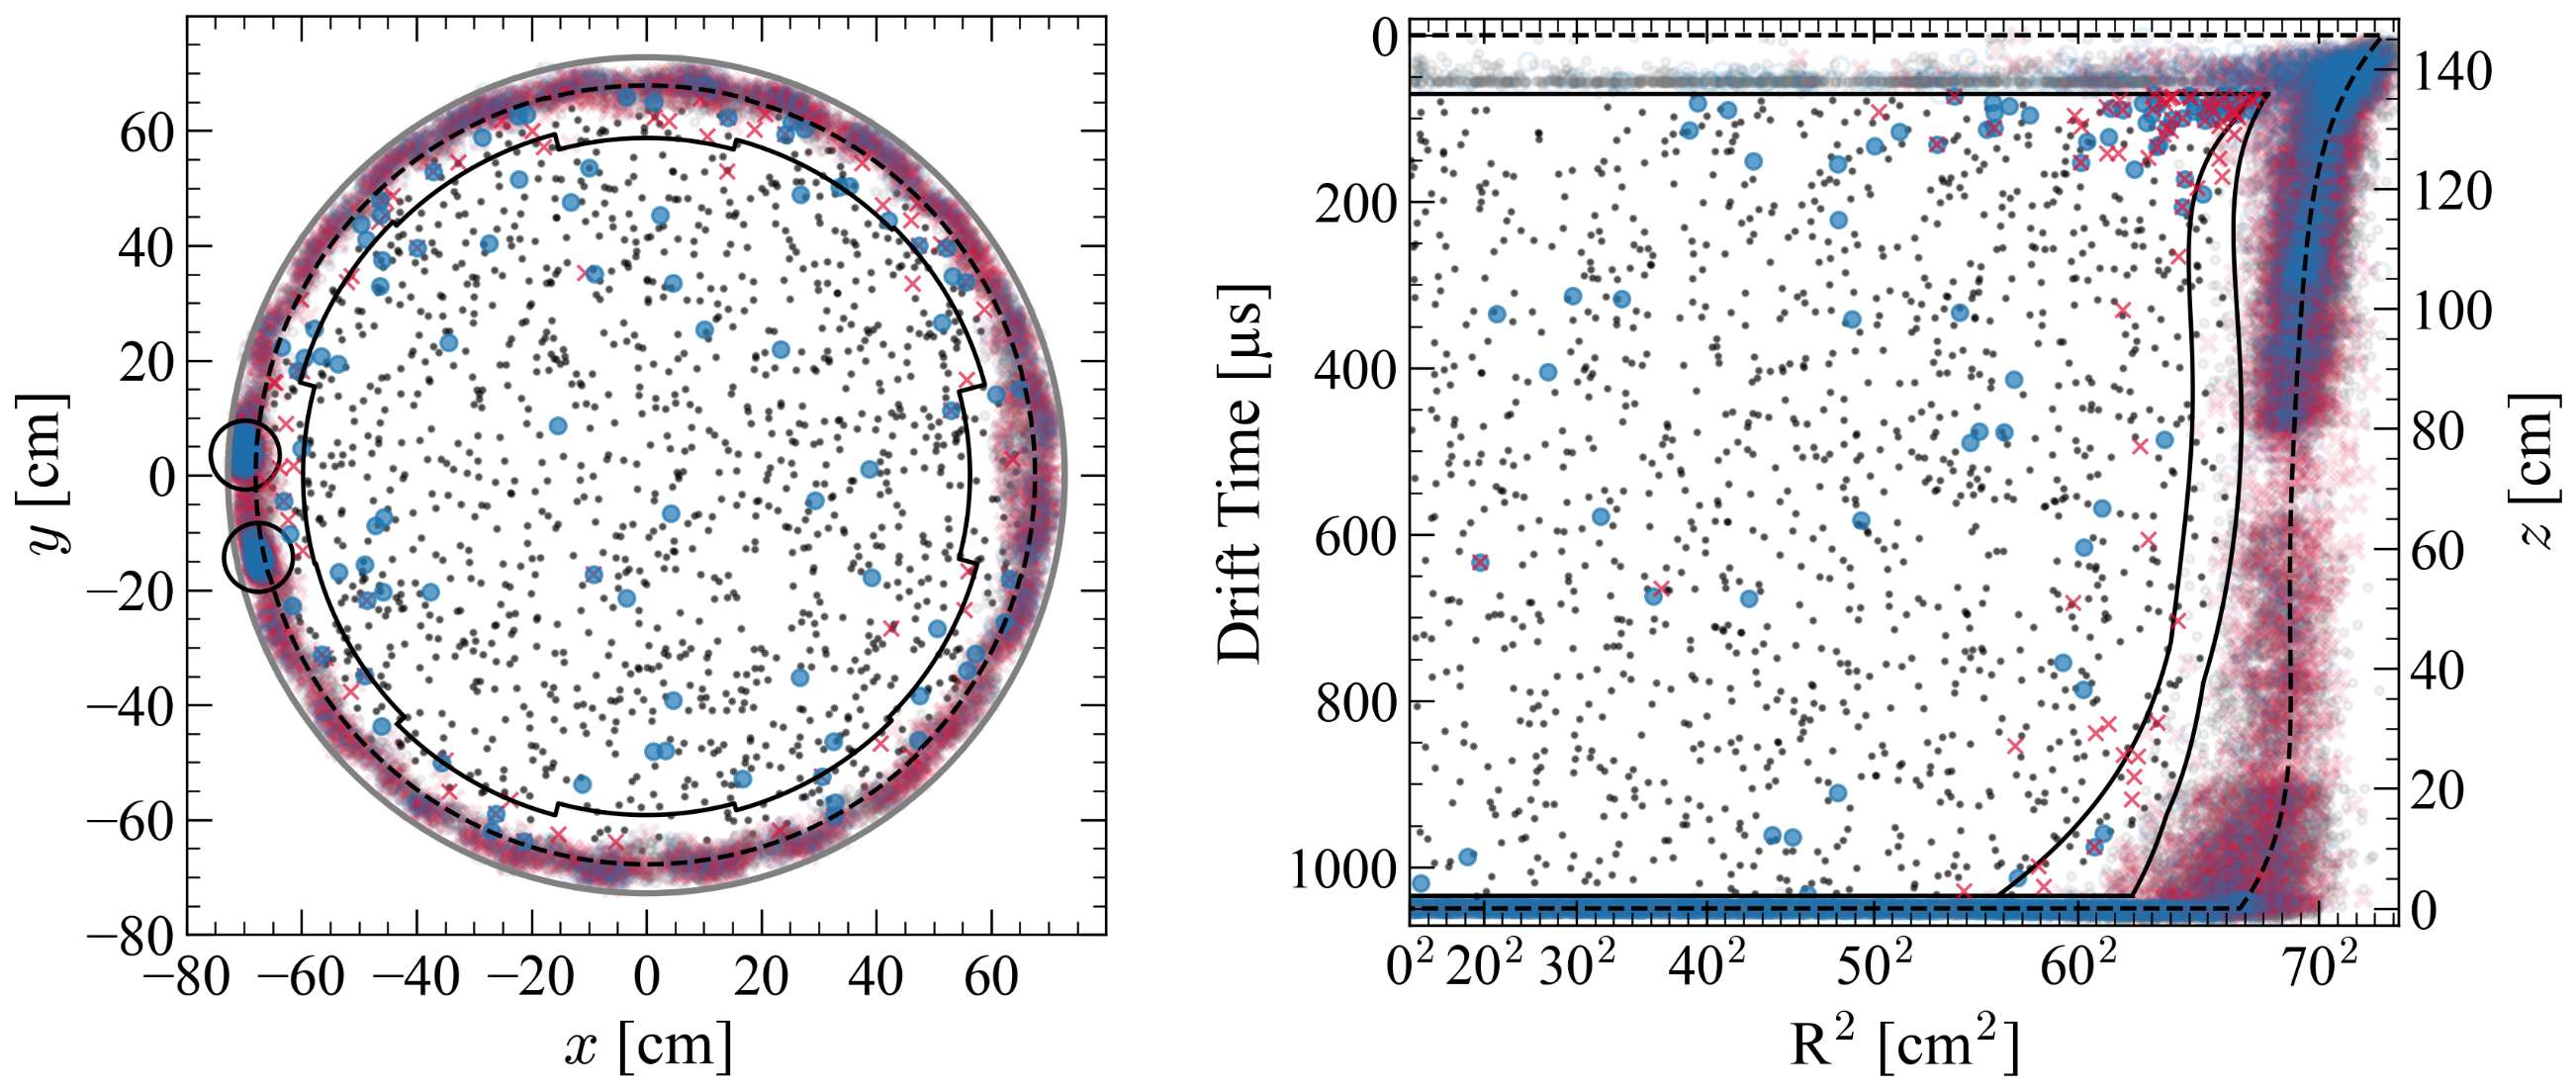
\includegraphics[width=\linewidth]{figures/VetoEfficiency/WS2024_TPCPosPlots_2panel.png}
    \caption{\textbf{Left:} Data from the WS2024 science run reconstructed in TPC $x$ and $y$ position, in black with all analysis cuts applied. Red crosses and blue circles represent events that are vetoed by the Skin and OD veto coincidence cuts, respectively. The dashed line shows the active volume, averaged over azimuth, and the solid lines depict the FV, at the azimuths of its smallest and largest radial extent. The two circle lines depict the boundary of the position based selection which remove events within 6~cm of TPC field cage resistors with elevated rates of radioactivity. \textbf{Right:} The same events shown in the left panel in reconstructed in TPC $\text{R}^2$ and $z$.}
    \label{fig:VetoEff/WS2024_TPCPosPlots_2panel}
\end{figure}

Events which have a coincidence signal in the delayed veto window have a higher chance to have been caused by a neutron recoiling in the TPC. Selecting events with a veto signal therefore yields a neutron rich sideband with which we constrain the neutron rate in the WIMP 2024 data set.
Events which passed the Skin-delayed and OD-delayed selection are used to generate the side band sample. In the final statistical analysis, a likelihood fit returns an expectation of $0.0^{+0.2}$ SS counts attributed to detector neutrons \cite{LZCollaboration:2024lux}. The events selected for this side band analysis are shown in \autoref{fig:VetoEff/VetoSideBandEvents} and are overlaid against the final set of events passing all selection cuts. 

\begin{figure}[ht!]
    \centering
    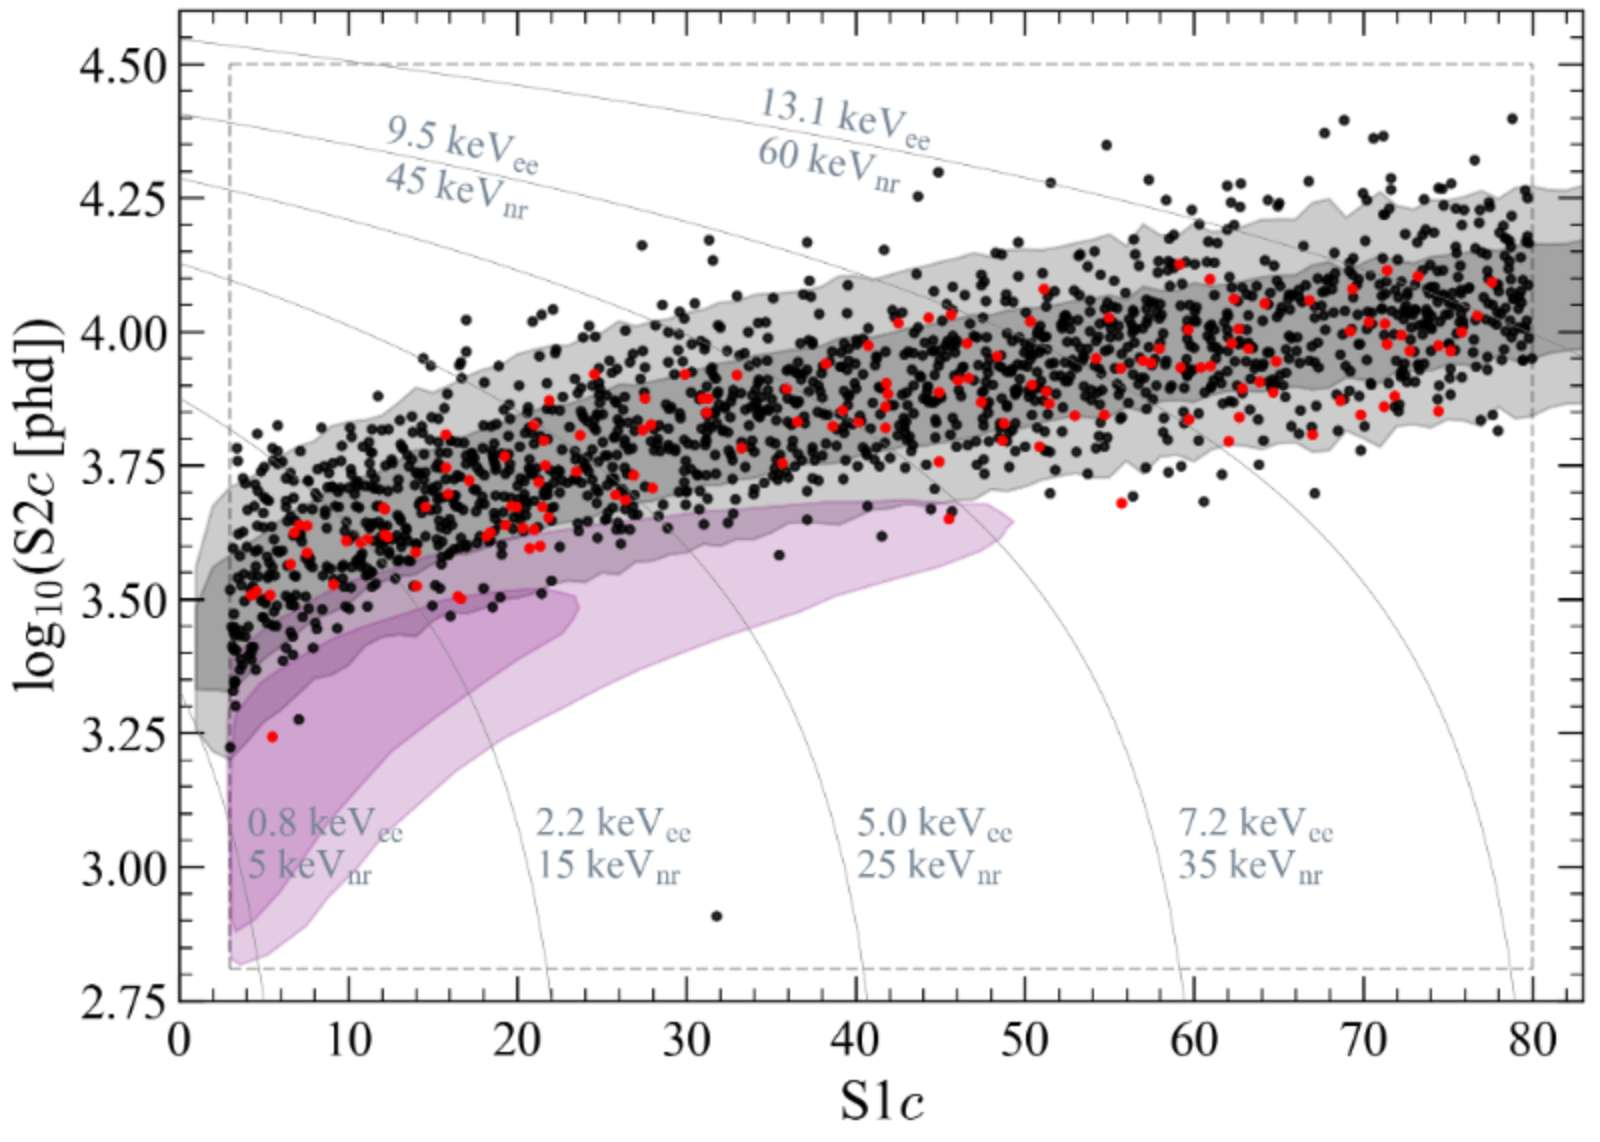
\includegraphics[width=0.7\linewidth]{figures/VetoEfficiency/WS2024VetoSideBandEvents_WIMP40.png}
    \caption{The final set of events passing all selection cuts are shown in black. Events that are tagged by the Skin and OD delayed selection are shown in red. Regions containing 68\% and 95\% of the ER portion of the background model and a 40~GeV/$c^2$ WIMP are shown with the dark and light gray and purple shading respectively. Gray lines show contours of constant ER-equivalent ($\text{keV}_\text{ee}$) and NR-equivalent ($\text{keV}_\text{nr}$) energy. The dashed lines shown boundary of the WIMP region of interest.}
    \label{fig:VetoEff/VetoSideBandEvents}
\end{figure}

\section{Concluding remarks}
Improvements to the Outer Detector geometry in simulation now better reflect the neutron capture timing observed in calibration data sets. As the time between single scatter S1 and veto pulses is considered in the veto coincidence selection, the accurate modelling of the detector response in simulation is crucial for the optimisation of veto coincidence selection for the WIMP analysis. These improvements are further reflected in the measurement of the neutron tagging efficiency when results are compared to simulations of AmLi and DD calibration sources. The optimisation of the veto coincidence selection resulted in a factor of two reduction in detector dead time induced by the selection whilst maintaining the same tagging efficiency measured in the WS2022 science run. An estimated neutron tagging efficiency of $(92\pm4)\%$ with a 3\% detector dead time is presented. The inclusion of the veto coincidence selection to the WIMP analysis cuts affords LZ the ability to increase the fiducial volume by 40\% by rejecting background events near the wall of the TPC which otherwise would be removed by constraining the fiducial volume selection. To estimate the number of single scatter events resulting from detector neutrons, a sample data set of events selected using the delayed veto coincidence selection is generated. An expectation of $0.0^{+0.2}$ single scatter events are attributed to detector neutrons using likelihood fit analysis. It should be stressed that if a WIMP signal were observed by LZ, the veto system will be crucial to excluded backgrounds as an explanation for the excess. To conclude this chapter I echo the words of Carl Sagan, \textit{``extraordinary claims require extraordinary evidence''} \cite{SaganCarl:BrocasBrain}.